\documentclass[12pt,a4paper]{report}
\usepackage[utf8]{inputenc}
\usepackage[T1]{fontenc}
\usepackage[czech]{babel}
\usepackage{graphicx}
\usepackage{booktabs}
\usepackage{hyperref}
\graphicspath{{./assets/}}

\usepackage{url}
\author{Michal Žáček}
\title{{\Huge Blender pro Smrtelníky}\\ {\Large Příručka k Blenderu v2.8} \\ {\large Ročníková Práce}}
\date{2019/20}

\pagestyle{headings}

\begin{document}
		\maketitle
	\pagebreak
	{
		\centering
	{\Huge MENSA GYMNÁZIUM, o.p.s.} \\
	{\Large ROČNÍKOVÁ PRÁCE} \\
	
	\textit{Strukturalizovaná příručka k 3D Grafickému programu Blender}
	
	{\large Obor: Počítačová Grafika
\\
		Autor: Michal Žáček \\}
	}
	\begin{itemize}
	\item[] Třída: Septima
	\item[] Školní rok: 2019/20
	\item[] Vedoucí práce: Hana Šromová
	\item[] Oponent/Konzultant: Dominika Lippertová
	\item[] Rozsah práce (s.):
	\begin{itemize}
		\item[] celkový (včetně této strany, vyjma titulní): 
		\item[] vlastní text:
		\item[] vědecký aparát (poznámky, bibliografie aj.):
	\end{itemize}
	\item[] Formát elektronické podoby práce: PDF
	\end{itemize}
\begin{abstract}
	\paragraph{Anotace} Tato práce se snaží namísto obvyklých internetových tutoriálů přiblížit. Blender jako software systematicky a s mnohými okolními znalostmi,
	které jsou potřebné k jeho plnému využití. Snažím se předat znalosti
	tak, aby čtenář pochopil logiku, na které stojí úkony, které provádí a
	byl schopen vyvozovat z nich závěry, pomáhající při dalším rozvíjení a
	používání programu.
	\paragraph{Klíčová Slova} 3D Grafika, Blender, Příručka, Výukový Materiál
	\paragraph{Anotace (AJ)} This work tries instead of the usual internet tutorials to approach
	Blender as a software systematically and with many surrounding
	knowledge that is needed to fully use it. I try to pass on the knowledge
	in such a way, that the reader understands the underlying principles on
	which the actions he performs stand and so that he may later be able
	to draw conclusions from them, helping to use and develop their use of
	the program.
	\paragraph{Klíčová Slova (AJ)} 3D Graphics, Blender, Handbook, Educational Material
\end{abstract}
	\pagebreak
	\tableofcontents
	\pagebreak
	
	\chapter{Předmluva}
	\section{Informace o Dokumentu - Cílová Skupina, Styl a Záměr}
	Psáno pro Blender 2.8. Tento dokument má zahrnovat základní znalosti
	potřebné k rozumné práci ve 3D grafických programech se zaměřením na
	Blender.
	Je důležité vědět, že cílem této práce je seznámit čtenáře s Blenderem do
	takové míry, aby byl schopen sám začít prozkoumávat tento rozsáhlý
	program. Mnohé části jsou přeskočeny nebo vysvětleny povrchně za
	účelem nezahltit čtenáře.
	Účelem je vysvětlit, jak funguje Blender spíše v jeho principech a s
	některými nuancemi, které mohou nováčkům dělat problém. Je mnoho
	lidí, kteří se již do modelování v Blenderu chtěli pustit, ale poté, co si našli
	na internetu nějaké tutoriály, stejně nevěděli, co dělali, protože jenom
	slepě sledovali tutoriál bez hlubšího pochopení. Pochopení problematiky,
	schopnost stavby na předešlých znalostech a zkoušení si sám nových
	věcí, je stav, který je právě záměrem této práce.
	\section{Kde všude se používá}
	„Používám Blender protože je silný, ne protože je zdarma“, řekl Max
	Puliero v rozhovoru s CGCookie.com v roce 2017. \cite{cgcookiePuliero} Od té
	doby, především během několika posledních pár let, se Blender přeměnil
	z komerčně téměř nepoužívaného programu v extrémně výkonný kus
	softwaru, který by mohl konkurovat mnohým placeným alternativám.
	Příklady, kde Blender byl použit:
	Max Puliero uvedl, že při práci na hře Dark Souls III, používal na design
	postav Blender, přestože jeho studio standartně užívalo jiné programy.
	\cite{cgcookiePuliero} Ubisoft Animation Studio má v průběhu roku 2020
	adoptovat Blender jako svůj hlavní software. \cite{ubisoft-news-BlenderDevFund} Unity Game
	Engine nativně podporuje [.blend] soubory.
	Již dlouho existovaly filmy tvořené pomocí Blenderu, ale Next Gen (2018)
	od Netflix je jeden z prvních komerčních filmů, které byly skutečně
	animovány čistě v Blenderu (Veldhuizen, 2018). Pokud nebereme celý
	film, ale stačí využití, pak ve filmu Warcraft (2016) byl narychlo přidán
	Murloc s jeho pomocí. (Failes, 2016)Pokud se zajímáte spíše o vesmír, NASA vydala některé z jejích modelů
	v [.blend] formátu. Dokonce projekt Experience Curiosity nějakou dobu
	běhal na Blender Enginu, dokud nebyl zrušen.
	Takže jak sami vidíte, není toho málo.
	\begin{figure}
		\centering
		\includegraphics[scale=0.25]{next-gen.jpg}
		\caption{Next Gen Film \cite{netflix-nextgen}}
		\label{pic:netflix-nextgen}
	\end{figure}
	
	\section{Blender Foundation - Trocha Historie \\ \cite{wikiBlender}}
	\begin{figure}[h]
		\centering
		\includegraphics[scale=0.3]{Ton-Roosendaal.jpg}
		\caption{Ton Roosednaal \cite{ton-roosendaal}}
		\label{pic:ton-roosendaal}
	\end{figure}
	
	\begin{figure}[h]
		\centering
		\includegraphics[scale=0.45]{man03.jpg}
		\caption{Blender circa 2002 \cite{blender-man}}
		\label{pic:blender-man}
	\end{figure}
	NeoGeo bylo dánské animační studio, které roku 1994 začalo vytvářet
	Blender pro firemní použití. Hlavním autorem byl Ton Roosendaal –
	tehdejší spolumajitel firmy. V roce 1995 už měli funkční verzi 1.0 a 1.
	ledna 1998 byl jejich program vydán jako freeware – volně dostupný na
	internetu. Ještě ten samý rok byla firma NeoGeo zanikla a Roosendaal
	založil svoji vlastní firmu Not a Number Technologies (NaN), za účelem
	dále rozvíjet projekt Blender. NaN roku 2002 zkrachovala a Roosendaal
	ještě téhož roku založil neziskovou organizaci Blender Foundation.
	Blender Foundation se během následujících let pokoušel udělat Blender
	Open-Source (prozatím byl Blender pouze volně dostupný jako celý
	program, open-source znamená, že bude i volně upravitelný a bude na
	něm moct pracovat kdokoli). Roosendaal vybral svůj cíl 100 000 euro od
	lidí a dosáhl svého cíle. Dodnes je Blender vyvíjen hlavně jeho komunitou
	a čtyřmi programátory zaměstnanými u Blender Foundation.
	
	\section{Blender není jen na 3D modelaci}
	Ačkoli začal svůj život jako animační program, vyvíjen pro potřeby
	animace, rozsáhlá komunita mu přidala množství různých dalších funkcí.
	Dnes zvládá editovat video, zvuk, zvládá sledovat objekty na kameře a
	nedávno se objevily i fotogrammetrické pluginy. Rozšířila se také podpora
	jiných programů. Není vzácné, aby herní engine měl podporu pro
	proprietární [.blend] soubory nebo podporoval přímé napojení pomocí
	pluginů.
	
	\section{Pluginy}
	Roztroušenost vývoje donutila Blender využívat tzv. pluginy. Plugin je
	funkce programu taková, že není brána jako součástí jeho jádra, ale bere
	se jako jeho rozšíření. Lze jej například i vypnout nebo stáhnout z
	internetu. Příkladem je třeba podpora dalších formátů, předpřipravené
	nové objekty a zjednodušený přístup k některým nastavením. Takových
	pluginů je obrovské množství a dají se doinstalovat do Blenderu podle
	potřeby. On sám už nějaké obsahuje, a i když jsou některé v základu
	vypnuty, není kolikrát potřeba je stahovat a lze je pouze zapnout v
	nastavení.
	
	\chapter{Interface}
	Blender se s pomocí své rozmanité funkčnosti snaží poskytnout co nejvíce
	možností a do toho je musí udržet přístupné a přehledné. K tomuto
	využívá systém oken, o kterém si nyní něco můžeme říct.
	Když poprvé spustíte Blender, tak vypadá následovně.
	
	\begin{figure}[h]
		\centering
		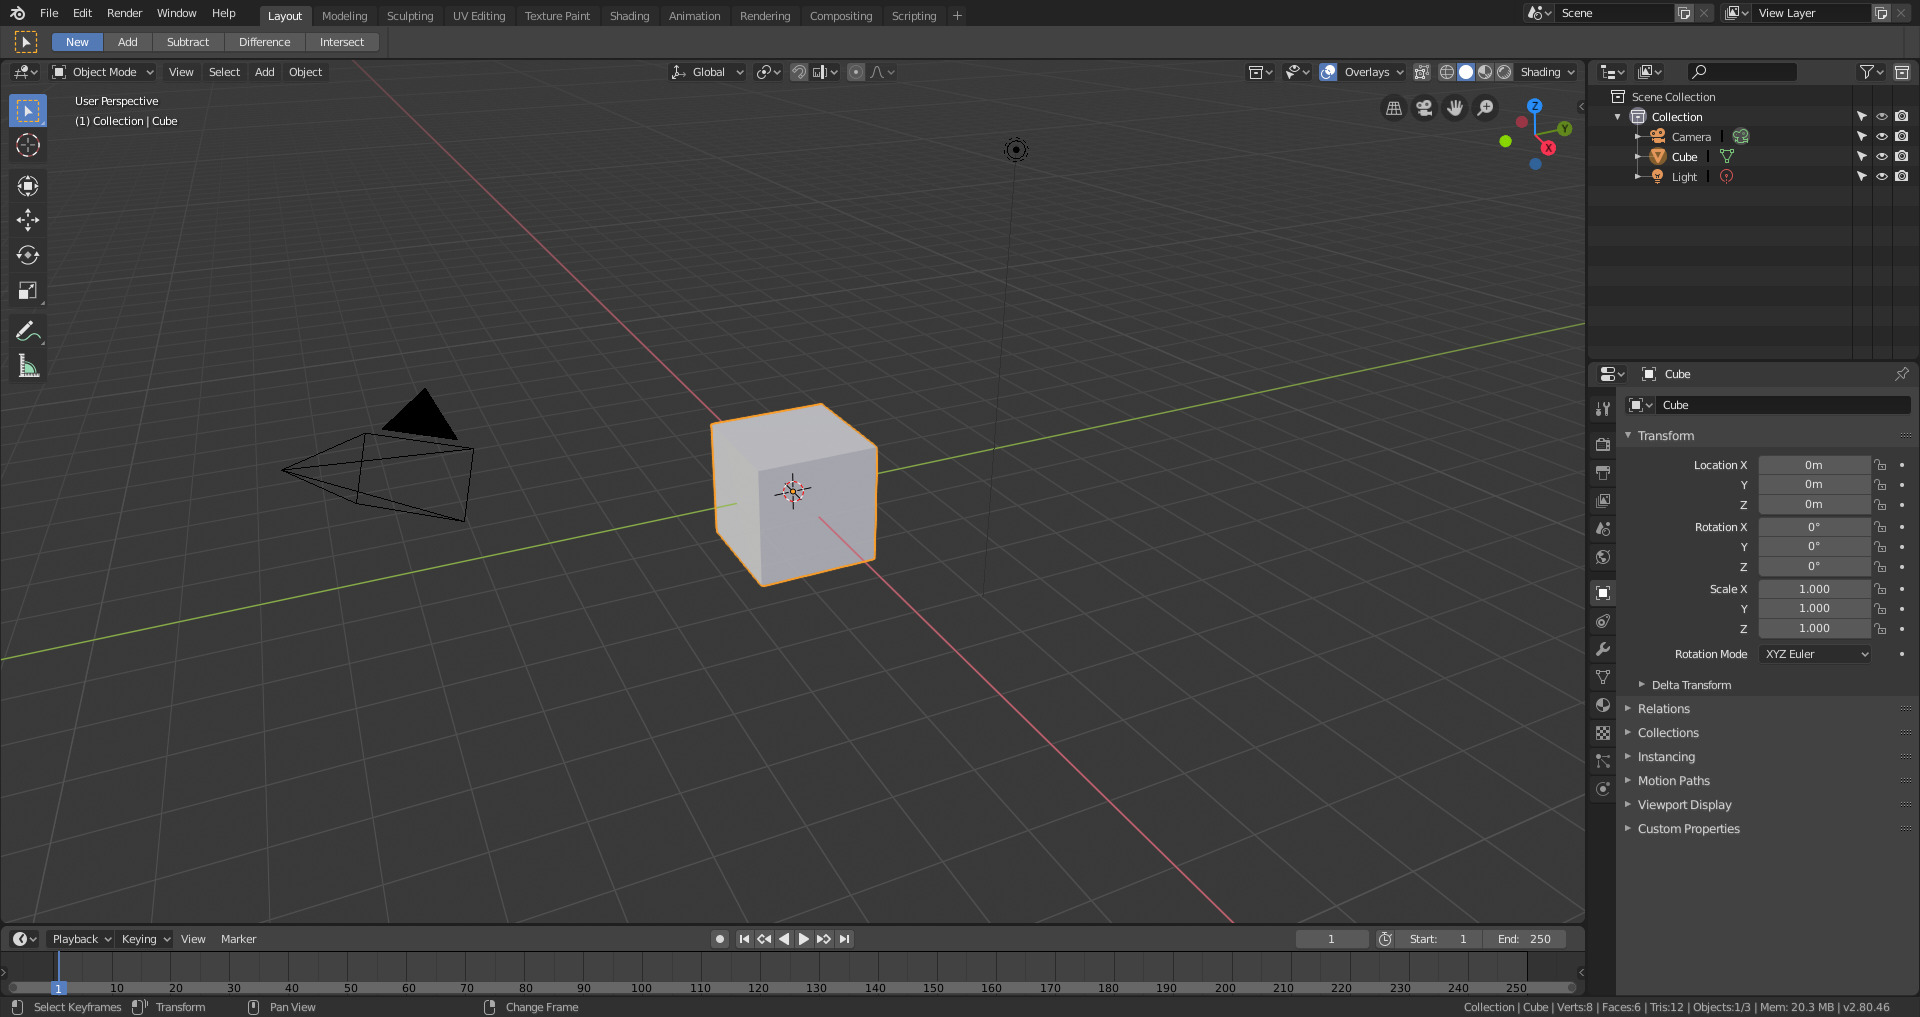
\includegraphics[scale=0.25]{ui/UI-1.png}
		\caption{Po spuštění}
		\label{pic:startup-1}
	\end{figure}

	Nejlépe je si přirovnat systém Blender k oknům u Vašeho počítače. Tak,
	jak máte na počítači otevřena mnohá okna vedle sebe (např.: prohlížeč,
	Word, mail atd.), stejně tak je to u Blenderu. Blender jako program má
	nespočet různých funkcí, které by byly absolutně nepochopitelné, kdyby
	byly ukázány všechny najednou. Proto jsou nástroje uvedeny do
	souvisejících oken, kdy každé z nich má sloužit k jednomu účelu -například okno pro umístění objektů do scény, okno pro jejich nastavení,
	okno pro editaci videa, okno pro práci s texturami atd.
	
	\begin{figure}[h]
		\centering
		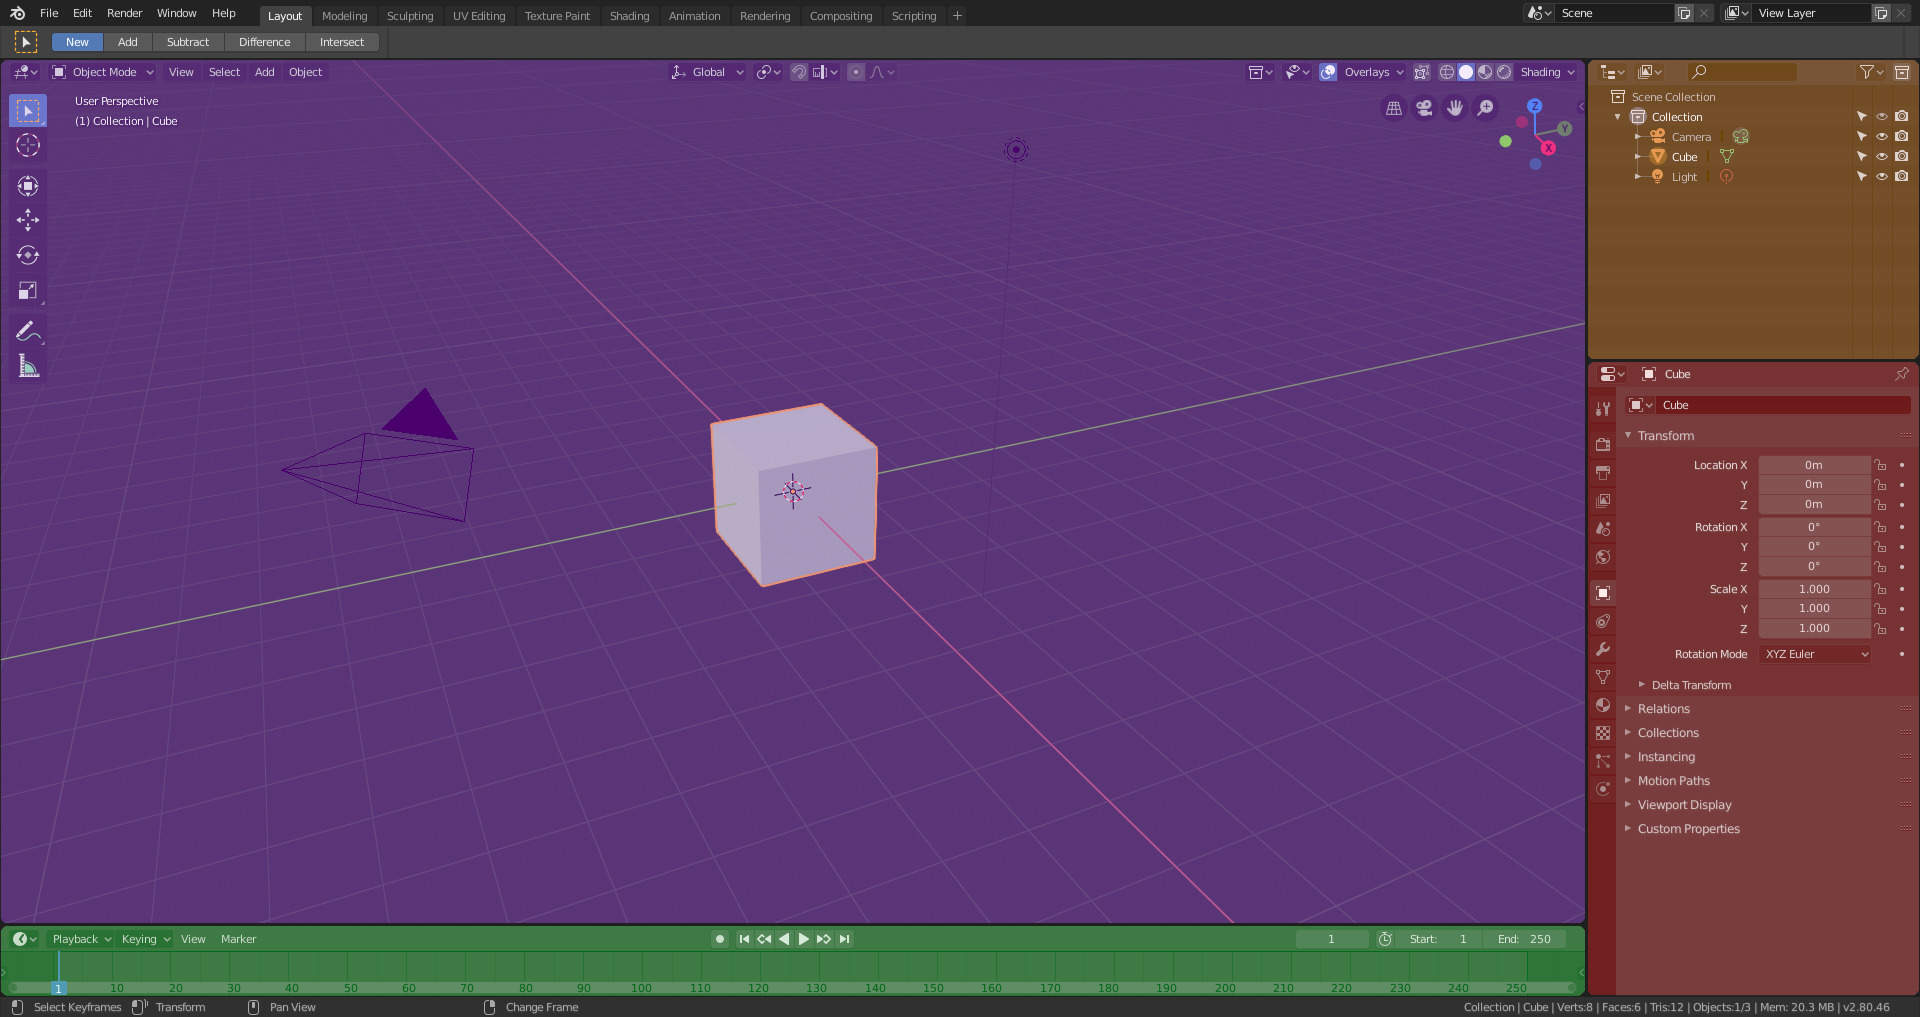
\includegraphics[scale=0.25]{ui/UI-2.png}
		\caption{Po spuštění (obarvené)}
		\label{pic:startup-2}
	\end{figure}

	Sledujme nyní obrázek \ref{pic:startup-2}. Modře je zaznačeno takzvané 3D zobrazovací
	okno, ve kterém budete pravděpodobně trávit nejvíce času. Zeleně je
	zvýrazněna Ćasová osa, která se používá hlavně při animacích. Napravo
	je červeně většina nastavení. Žlutě je Seznam objektů a skupin. Nakonec
	vršek lemuje informační panel, který obsahuje většinu ukládání, otvírání
	souborů a také se zde zobrazují procesy na pozadí jako vykreslování
	a fyzikální simulace.
	
	\paragraph{Pohyb s okny} Pokud najedete myší mezi dvě okna změní se Vám
	kurzor a můžete měnit jejich velikosti. Najetím na roh okna, kde se vám
	kurzor změní na kříž, je možné okna zavřít nebo otevřít.
	
	Obsah okna lze změnit v malém menu obsaženém v každém z oken. Na
	začátku jsou nejlépe vidět dva v obou rozích levé strany programu.
	Poznají se podle obrázku, vedle nějž se nachází šipka dolů. Po kliknutí na
	toto menu se Vám otevře výběr všech druhů oken, které si nyní
	projdeme.
	
	\begin{figure}[h]
		\centering
		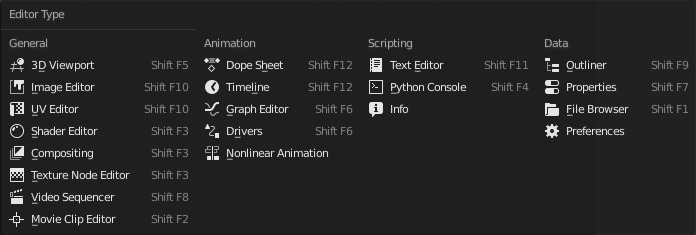
\includegraphics[scale=2]{ui/UI-WINDOWS.png}
		\caption{Výběr oken}
		\label{pic:windows-selection}
	\end{figure}

	\section{3D Zobrazení}
	
	Zde budou Vaše oči trávit nejvíce času. Okno 3D zobrazení Vám zobrazuje
celou scénu. Můžete v něm nejjednodušeji přepínat mezi objekty,
modelovat je, pohybovat a točit s nimi. Také se Vám zde promítnou
veškeré změny z jiných oken. Dále v něm můžete nahlížet do kamer
a vidíte v něm, jak vypadá Vaše scéna.
K pohybu v 3D zobrazení slouží nejlépe numpad. Klávesy 4, 8, 6 a 2 otáčí
	kameru kolem aktuálního středu. Stejný pohyb je dosažitelný přidržením
kolečka myši. 1, 7 a 3 nastaví pohled dle globálních os - přesně na pohled
shora, ze strany nebo zepředu. 9 invertuje pohled o 180 stupňů, takže pohled
zepředu otočí na pohled zezadu. K přiblížení a oddálení pohledu slouží
Klávesy [$+$] a [$-$] nebo kolečko myši.
Klávesa [Shift] změní 4 a 6 na klávesy otáčející pohled ze strany na
stranu, jako byste nakláněli hlavu. [Ctrl] změní všechny směrové klávesy
tak, aby posouvaly pohled ze strany na stranu, bez rotace.
	
	\subsection{Módy}
	Uvnitř tohoto okna se nalézá několik módů. Nejdůležitější z nichž jsou
	objektový a editační. Tyto dvě možnosti máme oddělené a přepínáme
	mezi nimi stisknutím klávesy [Tab]. Další módy jsou přístupné z menu
	v levém horním rohu.
	
	\subsection{Objektový}
	Tento mód slouží především k pohybu objektů a jako mezikrok k dalším
	módům a oknům. V objektovém módu můžete libovolně zvolit kterýkoliv
	objekt, který poté v dalších módech a oknech budete editovat, protoževšechny ostatní módy vždy pracují pouze s tímto jedním zvoleným
objektem.
	Objekt zvolíte stisknutím levého tlačítka myši kdekoli na něm.
	Pokud chcete zvolit více objektů najednou, přidržte k jejich volbě [Shift].
	
	\begin{figure}[h]
		\centering
		\includegraphics[scale=0.75]{ui/translated-cube.png}
		\caption{Transformovaná Kostka (translace, rotace, škálování)}
		\label{pic:cube-positioning}
	\end{figure}

	\paragraph{Zvolení objektů} Žlutým okrajem je zvýrazněn zvolený objekt. Ten je
	zobrazován a upravován v ostatních oknech. Oranžově jsou zvýrazněny
	další zvolené objekty, na které se také budou aplikovat translace nebo
	seskupování či další hromadné úpravy. Hlavním zvoleným objektem je
	vždy objekt, který byl do výběru přídán jako poslední. Blender referuje ke
	všem zvoleným objektům jako Selected a k hlavnímu zvolenému objektu
	jako active. Klávesou [,] zacentrujete pohled na zvolené objekty.
	
	\begin{figure}[h]
		\centering
		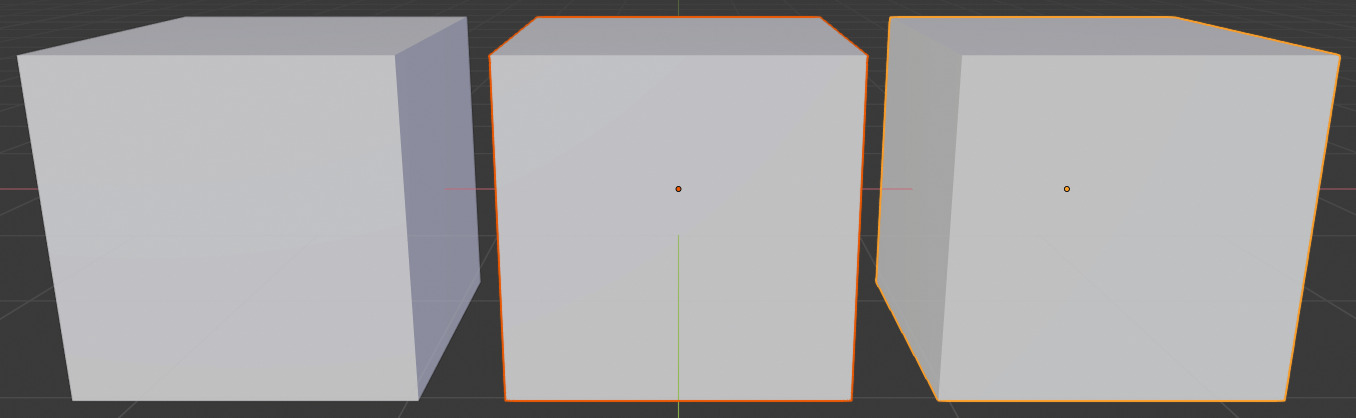
\includegraphics[scale=0.4]{ui/Selected-Cube.png}
		\caption{Volba objektů}
		\label{pic:cube-selection}
	\end{figure}

	\paragraph{Pohyb} Zde se rovnou hodí zmínit o klávesových zkratkách, těch má
Blender nespočetně, ale nyní jich budeme využívat jen několik. Nebojte,
bude to jednoduché.
	\newline \newline

	\begin{tabular}{cc}
		G & translace \\
		R & rotace \\
		S & rozměr
	\end{tabular}
	
	Poté, co jste zvolili, co chcete s objektem dělat, můžete říct přímo
	ve kterém směru. Tím, že stisknete jednu klávesu korespondující k jedné
	z os [X, Y, Z], změna se bude projevovat pouze na té ose. Pokud
	stisknete klávesu ještě jednou, tak zvolíte lokální osu namísto
	globální. Další stisknutí osu opět odemkne.
	Jsou tři osy pohybu - podle toho, k čemu jsou tyto osy kolmé, je dělíme
	především na lokální a globální. Lokální osa zahrnuje předešlé změny.
	Například krychle zobrazena níže má lokální osu X o 45 stupňů
	odkloněnou od globální osy X. Globální jsou totiž stacionární a vždy
	zůstávají stejné, osy X a Y jsou rovnoběžné s čárami zaznačenými kolem
	objektů, osa Z je na obě kolmá.
	Pokud chcete změnu provést o specifickou hodnotu, můžete ji napsat na
	klávesnici. Všechny změny se potvrzují levým tlačítkem myši a ruší se
	pravým.
	
	Příklad:
		\begin{figure}[h]
			\centering
			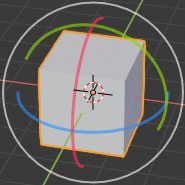
\includegraphics{ui/Rotary-Cube.png}
			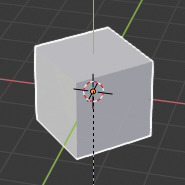
\includegraphics{ui/Rotary-Cube-1.png}
			\caption{Ukázka Rotace}
			\label{pic:cube-rotation}
		\end{figure}
	
	Když mám zvolený objekt, stisknu R, napíšu 45 a stisknu Z. Krychle se mi
otočí, jak vidíte výše, o 45 stupňů dle svislé osy Z.
	
	\begin{figure}[h]
		\centering
		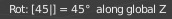
\includegraphics{ui/Rotary-Cube-2.png}
		\caption{Informace o změně}
		\label{pic:cube-rotation-2}
	\end{figure}

	Vlevo nahoře poté máme informace o současné probíhající změně, pokud
	ji chcete dodatečně měnit. Hodnotu lze dokonce standartně přepisovat
	klávesou [Backspace] a šipkami. Změna se potvrdí klávesou [Enter] nebo
	levým tlačítkem myši. Vráti lze klávesou [Esc] nebo pravým tlačítkem
	myši.
	Nové objekty lze přidávat z menu dostupného klávesovou zkratkou
	[Shift+A].
	
	\begin{figure}[h]
		\centering
		
\includegraphics[scale=3]{workspace/3DCursor.png}
		\caption{Výběr/3D Kurzor Spínač}
		\label{pic:3dcursor}
	\end{figure}

	\paragraph{3D Kurzor} Vlevo vidíte tento spínač, pokud je nastaven na spodní
	hodnotu, levé tlačítko myši namísto volení objektů, začne přemisťovat
	tzv. 3D Kurzor. Tento kurzor slouží k pár účelům. Jednak je to místo, kde
	se objevují nově přidané objekty, ale především slouží jako arbitrární
	přemístitelný bod v prostoru. Pomocí menu na zkratce [Shift+S] můžete
	přemístit 3D Kurzor na nějaké specifické místo nebo přemístit objekt na
	3D Kurzor.
	
	\paragraph{Origin} neboli počáteční bod, vyznačen na objektech malou žlutou
	tečkou, určuje jakousi jednotnou definici pro daný objekt. Protože objekt
	je často složen i ze stovek bodů, je potřeba jeden jasný bod, ke kterému
	lze referovat - například při zapisování jeho pozice. Pokud nahlédnete do
	vlastností objektu, vidíte zde pouze souřadnice jediného bodu, definující
	pozici celého objektu - tímto bodem je právě pivotový bod. Všechny
	transformace se také provádí se středem v pivotovém bodu, pokud není
	řečeno jinak. Nejlépe se nastavuje v menu Object > Set Origin.
	Na vrchu okna poté máte několik dalších nástrojů. Nejdříve popišme ty
	uprostřed.
	\paragraph{Pivotovým bodem} (Pivot point) se rozumí bod, vůči kterému jsou
	prováděny operace.
	
	\begin{figure}[h]
		\centering
		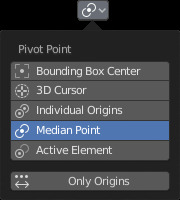
\includegraphics[scale=3.2]{workspace/pivot0.png}
		\caption{Menu pivotového bodu}
		\label{pic:pivot0}
	\end{figure}
	\begin{figure}[h]
		\centering
		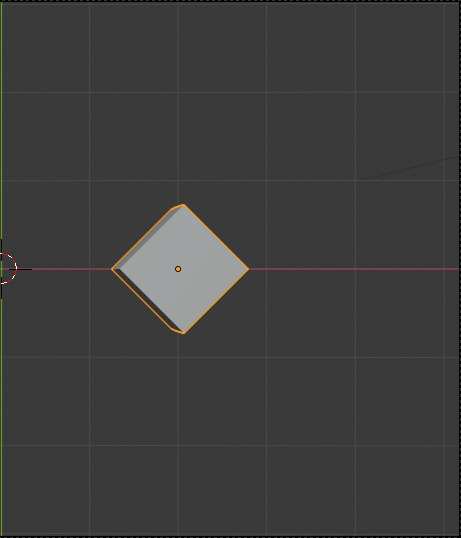
\includegraphics[scale=1.1]{workspace/pivot2.png}
		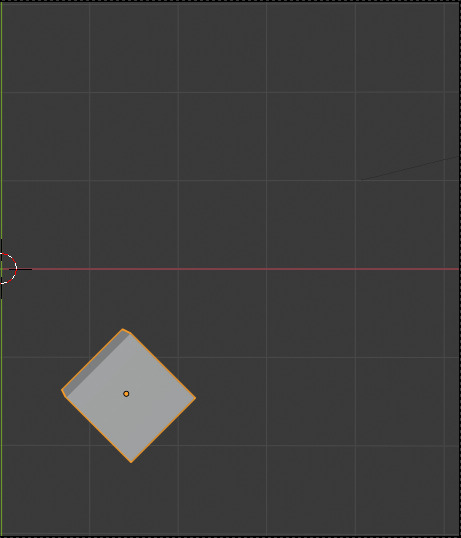
\includegraphics[scale=1.1]{workspace/pivot3.png}
		\caption{Ukázka pivotového bodu}
		\label{pic:pivot2-3}
	\end{figure}

	Například výše byly umístěny dvě krychle, jedna nalevo a jedna napravo,
	od středu na stejnou úroveň. Obě byly otočeny o 45 stupňů, ta vlevo kolem
	Originu a ta napravo kolem 3D Kurzoru.
	
	\begin{figure}[h]
		\centering
		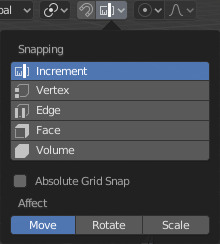
\includegraphics[scale=2.8]{workspace/Snap.png}
		\caption{Snap}
		\label{pic:snap}
	\end{figure}
	
	\paragraph{Snap} Další je menu něčeho nazývané Snap. Nejlépe by toto bylo
	přeloženo jako záchytné body. Magnetem se zapíná a vypíná, napravo
	vybíráte na co se změny chytají. Pokud máte například zapnutý Snap na
	Face, tak kdykoli provádíte změnu, například přemisťujete objekt, a vaše
	myš narazí na jakoukoli stěnu, objekt se na ni přichytí. Většinou to
	provede tak, že jeho nejbližší bod nastaví přesně na daný záchytný bod.
	
	\begin{figure}[h]
		\centering
		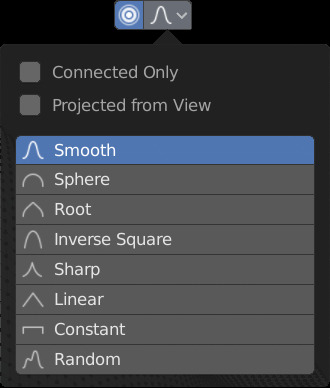
\includegraphics[scale=1.8]{workspace/Proportional0.png}
		\caption{Proporční}
		\label{pic:proportional0}
	\end{figure}

	\paragraph{Proporční editace} Při standartní editaci jsou ovlivněny pouze zvolené
	části (první obrázek níže), ale to často není co potřebujete. Proporční
	editace je vcelku jasná z názvu - ovlivňuje i nezvolené části meshe, silou
	odvíjející se dle jejich vzdálenosti od zvolených částí meshe. Pro zvětšení
	nebo zmenšení ovlivněné části točíte kolečkem myši. „Connected only“
	bude ovlivňovat pouze části meshe, které jsou direktně spojené se
	zvolenými částmi. „Projected from view“ určuje střed, od kterého se
	počítá vzdálenost, a následně tedy i síla změny pro daný bod. Pokud je
	vypnutý, změny se odvíjí od standartního středu definovaného pivotovým
	bodem. Pokud je zapnutý, střed je nejlépe popsán jako polopřímka
	začínající z místa vašeho pohledu a procházející pivotovým bodem.
	
	\begin{figure}[h]
		\centering
		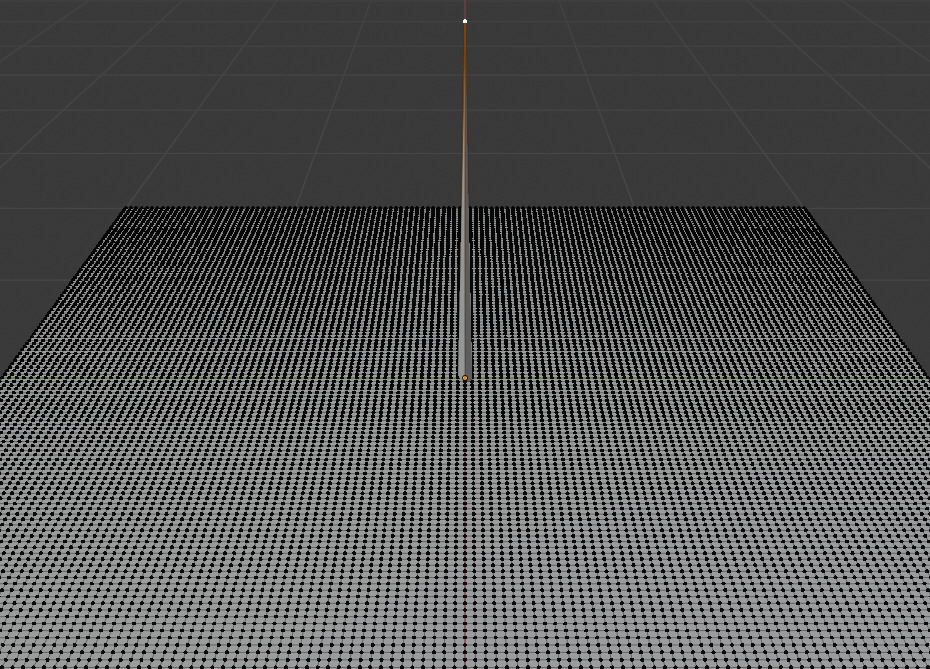
\includegraphics[scale=0.4]{workspace/Proportional1.png}
		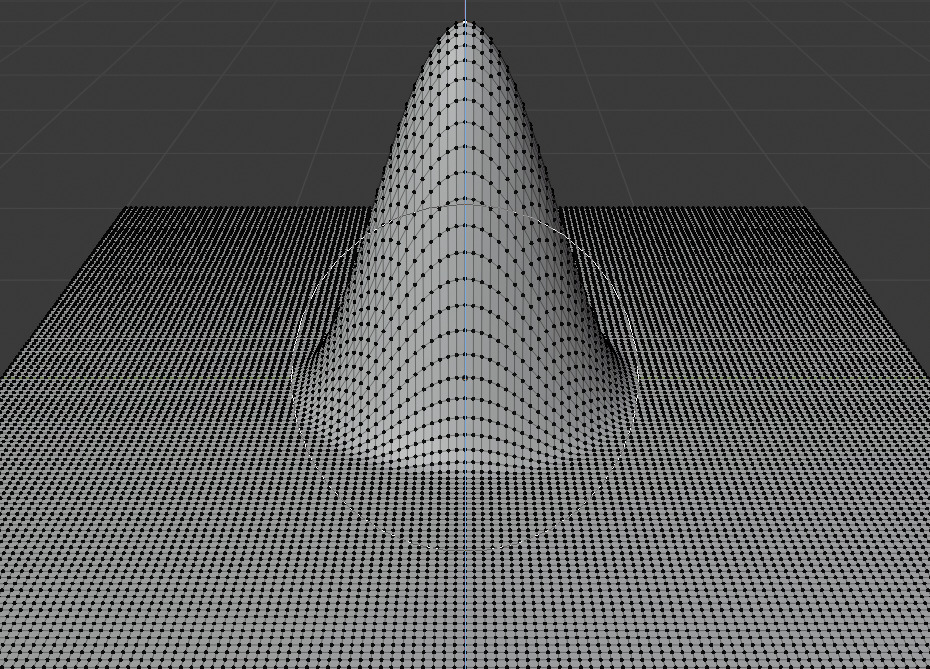
\includegraphics[scale=0.4]{workspace/Proportional2.png}
		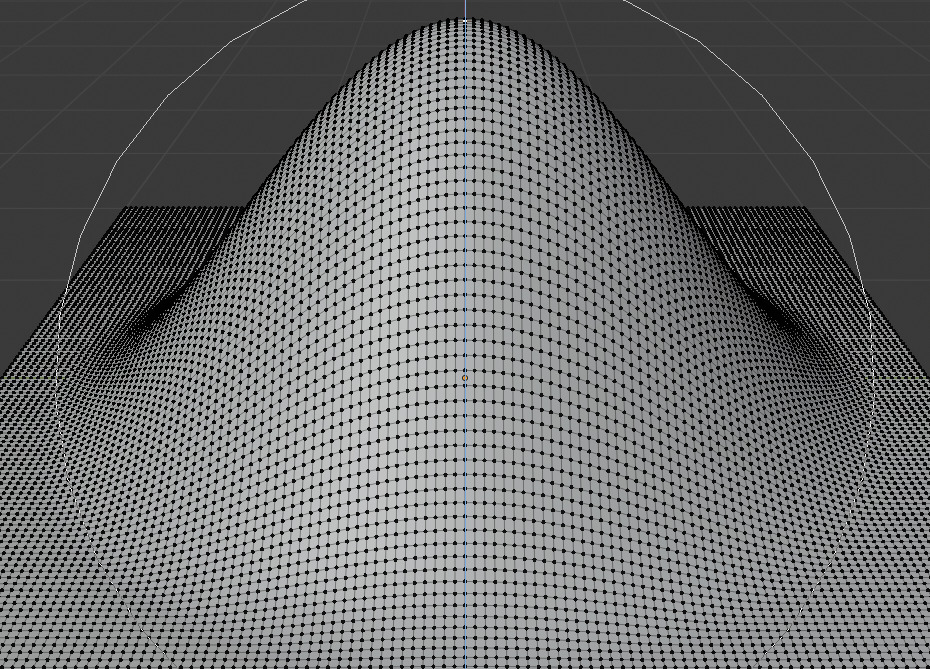
\includegraphics[scale=0.4]{workspace/Proportional3.png}
		\caption{Proporční editace (Bez, s, změna velikosti)}
		\label{pic:proportional1-3}
	\end{figure}

	\paragraph{/} Lomítkem schováte všechny nezvolené objekty. Opětovným
stisknutím je pak zase zobrazíte.
	
	\subsubsection{Editační}
	Zde - namísto editování celé scény, máte možnost zvlášť upravovat
	zvolený objekt včetně meshe. Zde můžete nastavovat i související věci
	jako [Vertex Group] nebo [Material], každé jednotlivé strany. \\
	
	\begin{figure}[h]
		\centering
		\includegraphics[scale=1]{workspace/selector.png}
		\caption{Výběr selekce}
		\label{pic:selector}
	\end{figure}

	V tomto menu si vybíráte, zda volíte roh, hranu nebo stěnu. Zatím
	nechme toto nastavené na stěny a ukažme si úkony, které lze dělat. Tyto
	jsou nejlépe ilustrované na stěnách, ale všechny platí také pro hrany
	a rohy.
	
	\begin{figure}[h]
		\centering
		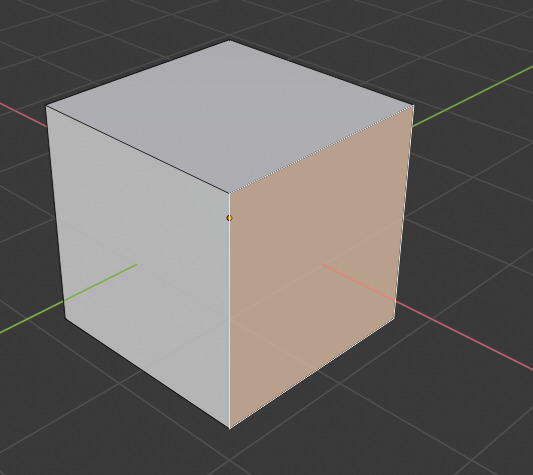
\includegraphics[scale=0.2]{workspace/Selection.png}
		\caption{Zvolená stěna}
		\label{pic:selection}
	\end{figure}
	\begin{figure}[h]
		\centering
		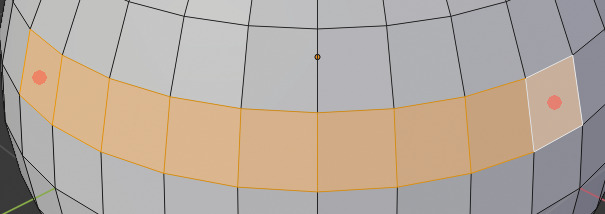
\includegraphics[scale=0.7]{workspace/CTRL.png}
		\caption{Výběr s klávesou [CTRL]}
		\label{pic:selection-ctrl}
	\end{figure}

	Volí se stejně jako u objektů - levým tlačítkem myši a přidržením [Shift]
	na zvolení více najednou. Rozdíl je, že hlavní zvolená stěna je zabarvena
	stejně jako ostatní, pouze je opatřena bílým obtažením.
	Máme zde navíc možnost zvolit „nejkratší“ cestu mezi dvěma body.
	Zvolíme počáteční a poté se stisknutým [Ctrl] zvolíme konečný bod.
	Kombinace [Alt + Shift] se pokusí nalézt jakousi cykličnost ve Vašem
	objektu a zvolit ji. Například pokud máte válec a stisknete na hranu jeho
	horní stěny, zvolí se celý okraj kolem dokola. Na obrázku \ref{pic:loop-cut} jsou tyto
	volby žlutě.
	Co se týká translace, rotace atd. vše je stejné jako u celých objektů.
	Fungují zde stejné zkratky a principy.
	
	\begin{figure}[h]
		\centering
		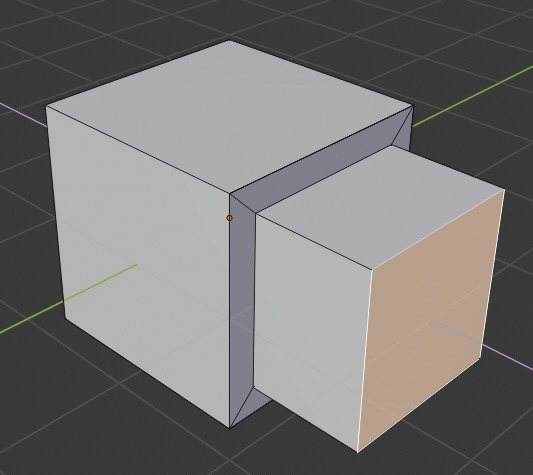
\includegraphics[scale=0.7]{workspace/Extrude.png}
		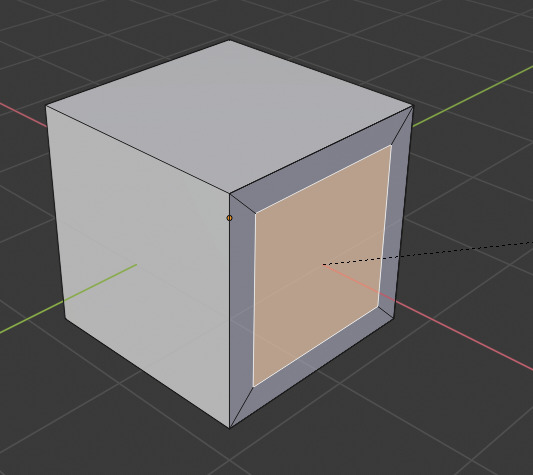
\includegraphics[scale=0.7]{workspace/I.png}
		\includegraphics[scale=0.7]{workspace/intrude.png}
		\caption{Inset, Extrude}
		\label{pic:edit-actions}
	\end{figure}

	Dva úkony, které slouží jako základ pro pokročilejší editaci, jsou Inset a
	Extrude. Nalezneme je na klávesách [I] a [E]. Inset vesměs utvoří novou
	stěnu napojenou stranami na tu původní a nechá Vás ji škálovat. Po
	stisku klávesy [I] a posunutí myši, Vám zůstane kostka z obrázku výše
	nalevo. Extrude udělá stejné napojení, ale posléze je nová stěna
	posunována, ne škálována. Tyto dvě operace lze aplikovat i na více stěnnajednou. Pokud jsou to stěny sousedící, akce bude provedena jako by se
	jednalo pouze o jednu stěnu.
	[Shift + A] funguje i v edit módu a přidá nový mesh do stejného objektu.
	Může se to zdát jako přidání nového objektu, ale všechny tyto části
	zastřešeny pod jedním objektem mají jediný Origin a sdílí mezi sebou
	všechny Omezovače a Modifikátory. Pro zvolení celé jedné spojené meshe
	je dobrá klávesová zkratka [Ctrl + L].
	
	\begin{figure}[h]
		\centering
		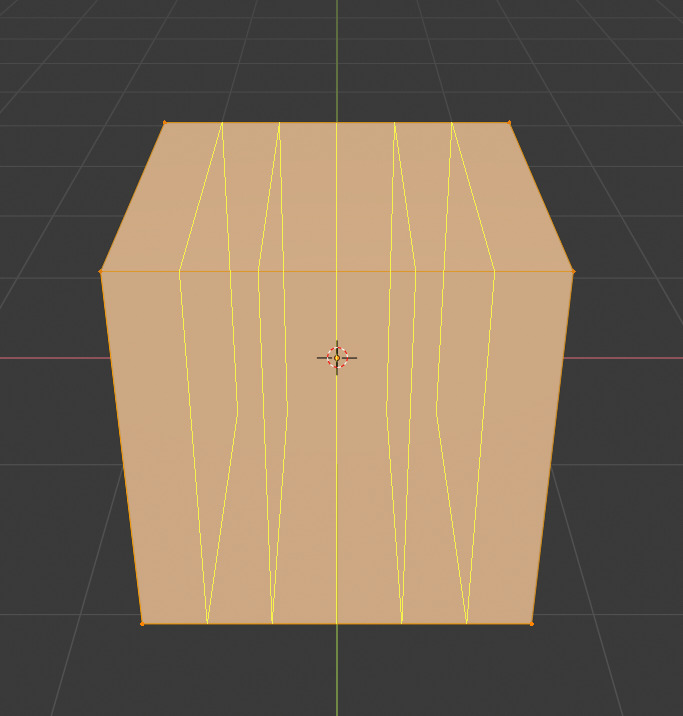
\includegraphics[scale=0.7]{workspace/Loop-Cut.png}
		\caption{Loop Cut}
		\label{pic:loop-cut}
	\end{figure}

	\paragraph{Loop Cut} Zkratkou [Ctrl+R] můžete provézt takovýto řez. Myší zvolíte,
	kde se má provést a napsáním čísla zvolíte na kolik částí takovýto řez
	rozdělí objekt. Výše bylo užito rozdělení na pět částí.
	
	\paragraph{Oddělování a Slučování} Stisknutím klávesy [P] se Vám otevře menu,
	ve kterém si můžete vybrat, dle čeho oddělíte část Vašeho současného
	objektu do objektu nového.
	
	\subsection{Kamera}
	
	\begin{figure}[h]
		\centering
		\includegraphics[scale=0.7]{workspace/camera.png}
		\caption{Kamera}
		\label{pic:camera}
	\end{figure}

	Stejně jako v realitě na scéně musí být kamera, která zaznamenává
	světlo odrážející se od scenérie. Pro vykreslování budeme většinou
	v Blenderu používat něco podobného. Pokud děláme cokoliv složitější než
	jeden model, který si otáčíme uprostřed obrazovky, je potřeba počítači
	říct, jak má scénu zobrazovat. Kamer může být více a každá obsahuje
	spoustu informací - například ohledně její pozice, rotace, perspektivy,
	objektivu a mnohé další.
	
	\subsubsection{Kamerový pohled}
	V [Okno 3D zobrazení] můžeme vidět buď volně nebo pohledem kamery
	Scéna má většinou nastavenou jednu kameru jakožto výchozí. Při stisku
	[Klávesy 0] je náš pohled nastaven na ten skrze výchozí kameru.
	[Ctrl+Alt+0] nastaví kameru na Váš aktuální pohled.
	\subsubsection{Důležitá nastavení}
	\paragraph{Lens}
	Pod nastavením čočky máte čtyři důležité možnosti:
	\begin{itemize}
	\item[Typ:] Perspektivní nebo Ortografická (viz. Perspektivy str.48)
	\item[Focal Length:] V podstatě optické přiblížení - zoom
	\item[Shift:] Toto se týká fotografického efektu zvaného Tilt-shift. Je moc
	náročné to zde vysvětlit, ale jsou na něj mnohé jiné zdroje.
	\item[Clip:] Říká kameře jaké rozpětí vzdáleností má zobrazit. Pokud je
	start nastaven na 10m a konec na 20m, kamera neuvidí nic blíženež 10m a vzdálenější než 20m. Pokud objekt leží přesně na
	hranici, zobrazí se pouze jeho část.
	\end{itemize}

	\paragraph{Viewport Display}
	Pro výsledek irelevantní, ale při práci velmi užitečný. Kamera je dosti
	komplexní záležitost a bylo by kontraproduktivní mít stále zobrazeny
	všechny informace o ní. Tady si vybíráme přesně ty, které chceme vidět
	v [Okno 3D zobrazení].
	\begin{itemize}
	\item[Size:] velikost ikony kamery
	\item[Limits:] zobrazuje odkud kam je nastaven [Clip]
	\item[Name:] pro účel přehlednosti větších kamerových sestav si můžeme
	vždy nechat zobrazit jméno kamery, jejíž pohled máme zobrazen
	\end{itemize}
	Toto nastavení má většina objektů. Má rozdílné parametry dle příslušného
	objektu, ale stejný účel.
	
	\section{Vlastnosti}
	
	Zobrazuje veškerá nastavení pro zvolený objekt a scénu. Například jeho
	lokace, užité materiály, fyziku atd. Pozor zobrazuje pouze hlavní zvolený
	objekt, nijak zde neovlivňuji sekundárně zvolené objekty (označeny
	oranžově).
	
	\subsection{Render}
	Popsáno v kapitole \nameref{section:render} str. \pageref{section:render}
	
	\subsection{Výstup (output)}
	\paragraph{Dimenze} (Dimensions) Resolution samozřejmě udává velikost
	výstupního obrazu. Hodí se zde poukázat na procentuální slider, neboť ve
	většině velkých projektů nebudete chtít vykreslovat v plné kvalitě hned od
	začátku, protože je to plýtvání časem - pokud potřebujete pouze rámcově
	zkontrolovat výstup.
	\paragraph{Aspect} mění skutečnou šířku nebo výšku pixelů - pokud nemáte jasný
	záměr, nechte zde 1:1.
	\paragraph{Render Region} Vám umožní renderovat pouze část obrazu. Toto
	nejlépe zvolíte v pohledu kamery zkratkou [Ctrl + B] a přetažením myší
	přes čtvercový region, který chcete renderovat.
	\paragraph{Frame Start a End} indikuje, od kterého do kterého časového bodu
	bude Blender renderovat. Můžete zde nastavit, abyste přeskakovali
	snímky.
	Ke \textbf{Frame Ratu} je třeba podotknout, že mění celkovou rychlost animace.
	Může tím pádem velmi změnit konečný vzhled animace, obzvláště
	v případech fyzikálních simulací.
	\paragraph{Výstup} (Output), zde se volí, kam a v jakém formátu chcete, aby byl
	výstup zapsán. Vesměs můžete vše nechat tak jak je, kromě File formátu.
	Pokud vykreslujete pouze snímek, na výběr máte standartní [.png],
	[.jpg], etc. Však pokud vykreslujete animaci, tak se spíše dává ve formě
	[.png], protože standartní video formáty mají problémy s přerušováním
	a úpravami uprostřed. Zkrátka pokud byste našli uprostřed nějakou
	chybu, museli byste začít Render od začátku. Pokud je Vaším formátem
	[.png], již vykreslené snímky Vám zůstanou a můžete poté pouze
	překreslit ty potřebné. Stačí najít kterou část je třeba překreslit a nechat
	renderovat jenom danou část. Jednoduché animace si pro pohodlí je
	samozřejmě možné vykreslovat do videa, ale udělat ze snímků video není
	těžké a je to možné udělat i v Blender oknu Video Sequencing.
	
	\subsection{Svět (World)}
	Navzdory prvotním pozorováním si všimneme, že není pozadí Vaší scény
	jen prázdný kanvas. Má materiál jako každý jiný objekt, využívá se
	převážně jako pozadí scény a pro osvětlení.
	Nastavit tento materiál lze pod Shader Editor > World.
	
	\begin{figure}[h]
		\centering
		\includegraphics[scale=0.7]{ui/world.png}
		\caption{Nastavení zvoleného objektu uvnitř Shader Editoru}
		\label{pic:world}
	\end{figure}
	
	Z mé osobní zkušenosti nedoporučuji u komplexnějších scén používat
	k osvětlení pouze Svět, protože toto světlo vypadá velmi uměle, neboť
	působí ze všech směrů identicky, což nevypadá dobře.
	
	\subsection{Object}
	Zde se nachází standartní data pro objekt - umístění rotace, velikost atd.
	Pokud chcete jednu osu uzamknout, aby se v ní s objektem nedalo
	manipulovat, učiníte tak stisknutím zámku vedle příslušné hodnoty.
	Následuje velké množství různých nastavení, která jsou důležitá, ale
	výrazně jednodušeji a přehledněji přístupná z jiných míst. Později se sem
	můžete vrátit. Pokud Vám tato zobrazení vyhovují více, můžete je také
	použít.
	Krom Viewport Display, kde volím, které informace o daném objektu se
	mi zobrazují ve [3D Viewport].
	
	\subsection{Materály}
	Popsáno v kapitole \nameref{section:materials} str. \pageref{section:materials}
	
	\subsection{Omezovače (Constraints)}
	
	\begin{figure}[h]
		\centering
		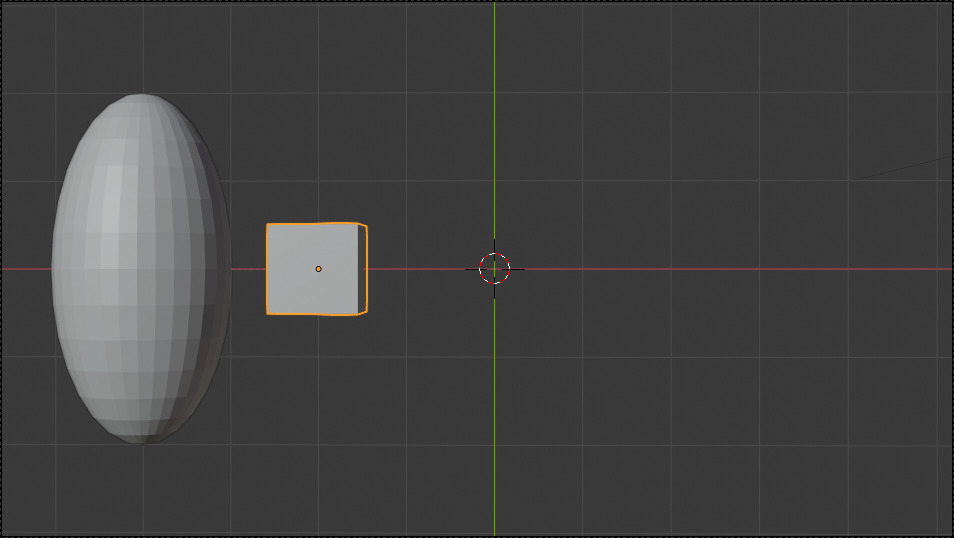
\includegraphics[scale=1]{constraints/limit-1.png}
		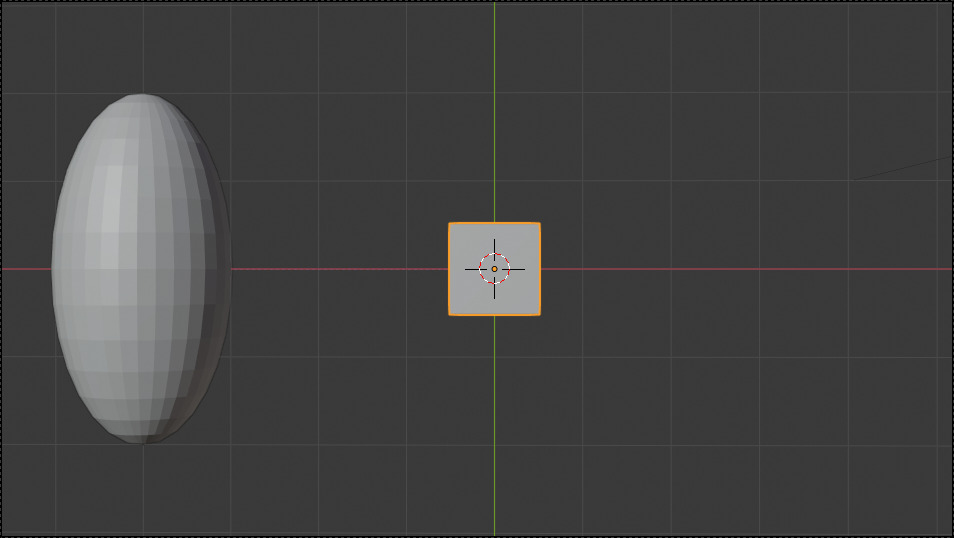
\includegraphics[scale=1]{constraints/limit-2.png}
		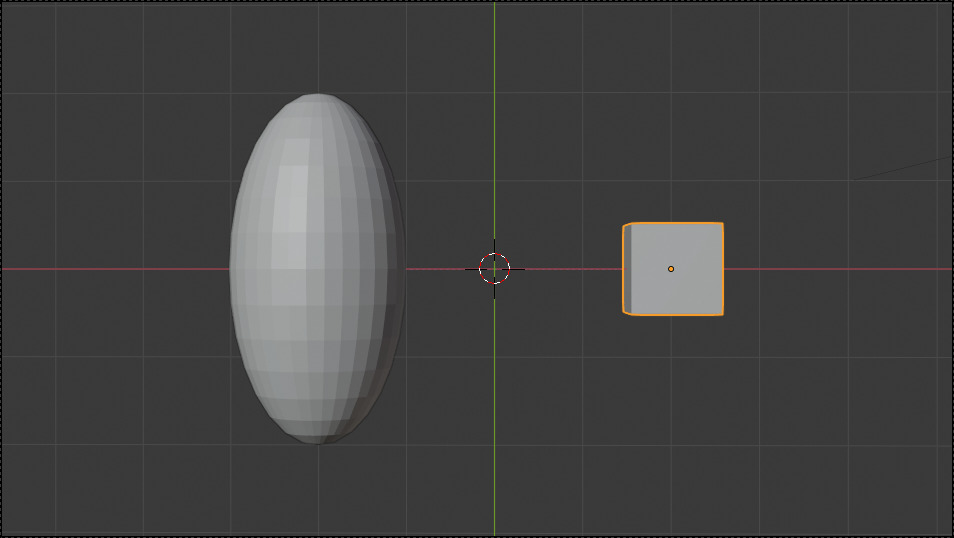
\includegraphics[scale=1]{constraints/limit-3.png}
		\caption{Aktivovaný Limit Distance Constraint na Elipsoid}
		\label{pic:constraints}
	\end{figure}

	Omezovače jsou definovaný vztah mezi dvěma objekty.
	Tyto vztahy sahají od kopírování rotace a pohybu po limitaci vzdálenosti
	mezi dvěma objekty. Aplikují se na objekt, se kterým se nehýbe – ten,
	který má být omezovačem upraven. Výše byl aplikován omezovač „Limit
	Distance“ na sféroid a s cílem na krychli. Nyní pohyb krychle zdánlivě
	pohne sféroidem, pokud je dostatečně vzdálená. Zdánlivě, protože jeho
	origin se nezmění, vypadá, že se pohnul, avšak pokud se podíváte do jeho
	vlastností, zjistíte, že jeho souřadnice se nezměnily.
	Často používaný omezovač je „Follow Path“, kdy definujete objektu cestu
	a čas, a on se po ní bude v daném čase pohybovat.
	
	\subsection{Modifikátory (Modifiers)}
	
	\begin{figure}[h]
		\centering
		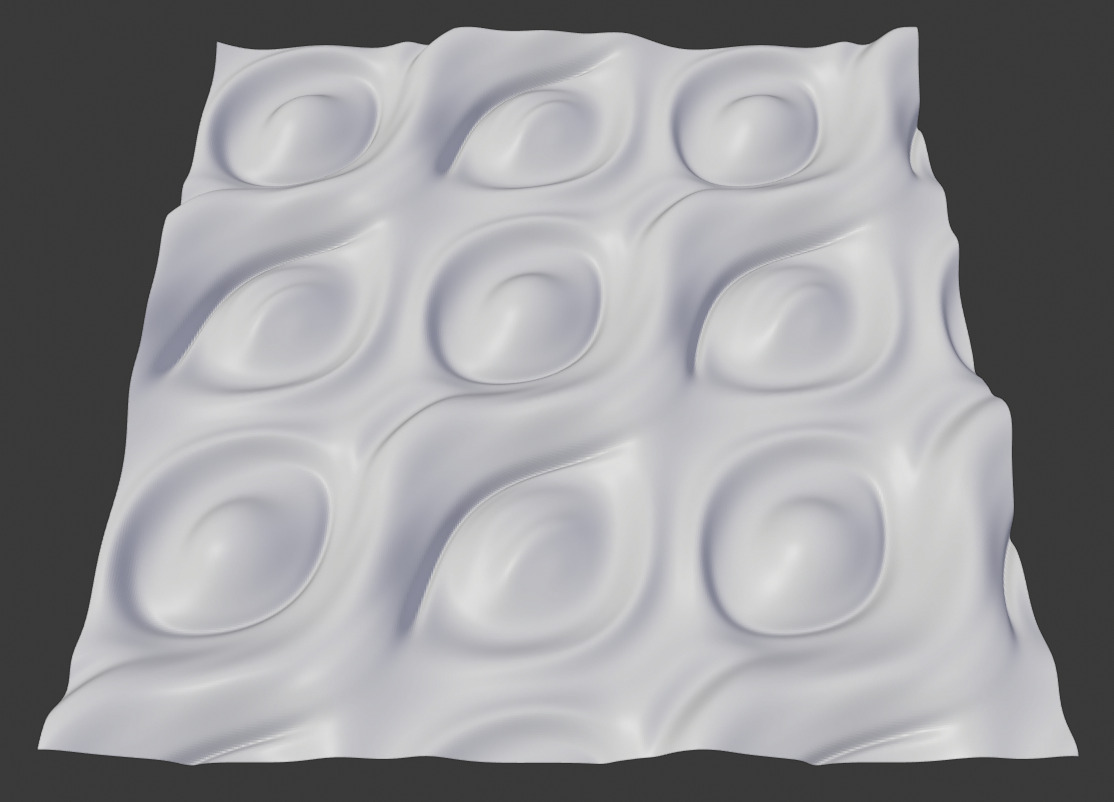
\includegraphics[scale=1]{modifiers/Modifiers-1.png}
		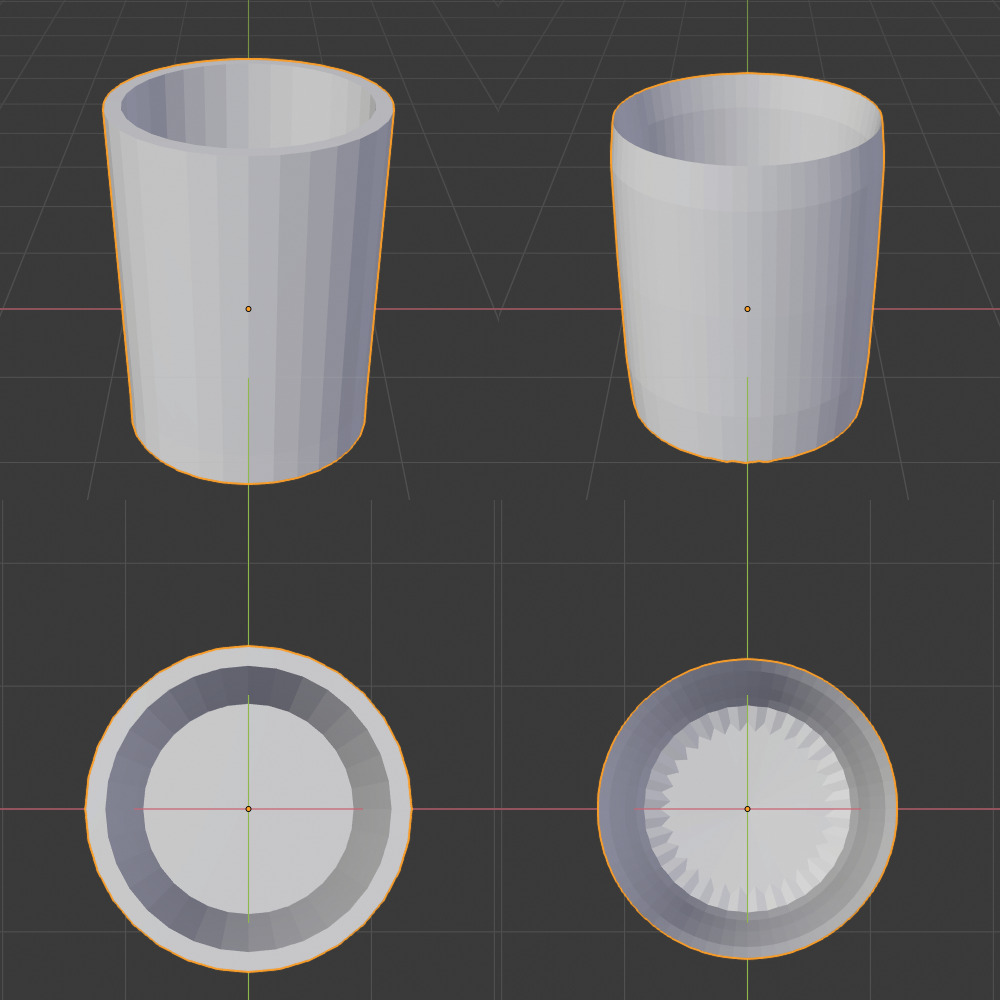
\includegraphics[scale=1]{modifiers/Modifiers-SSM.png}
		\caption{Ukázka Modifikátorů}
		\label{pic:modifiers}
	\end{figure}
	
	Modifikátory jsou procedurální efekty aplikované většinou na Mesh
	daného objektu. Jako příklady lze uvést nakopírování objektu za sebe,
	odečtení jednoho objektu od druhého, zarovnání rohů nebo zvýšení
	a snížení množství [Tri]. Celý smysl spočívá v tom, že tyto změny nejsou
	hned aplikovány, ale setrvávají na objektu. Takže pokud změním mesh,modifikátor se okamžitě přizpůsobí - dokud nestisknu Aplikovat, což
	natrvalo změní mesh a smaže Modifikátor. Modifikátorů mohu mít více
	najednou. Aplikují se vždy od vrchního tak, že každý následující pracuje
	již s meshem upraveným modifikátory předchozími.
	Nalevo je jednoduchá ukázka „Subsurface Modifier“, který se pokouší
	vyhlazovat meshe. Jako nafouknout uvnitř nich balónek a použít tento
	nový tvar jako tvar objektu. Napravo je pak kombinace „multiresolution“,
	který zvýší jednoduché ploše množství stěn, aby poté „displace“ mohl
	aplikovat z textury vzor.
	Nad nastavením každého modifikátoru, vedle jména, je nastavení
	zobrazení a dvě šipky, které vám umožňují posouvat jej nahoru nebo dolu
	v pořadí aplikování. Toto je důležité, protože například na obrázku výše
	napravo, pokud bych aplikoval nejdříve Displace, tak by se aplikoval na
	jednoduchý plain o čtyřech vertexech, což by akorát jeden z nich pozvedlo
	a Multiresolution by poté nebyl moc platný, protože by stejně zůstala
	placatá Plane.
	
	\subsection{Data > Vertex Groups}
	Pokud potřebuji označit určitou část objektu – například, aby měla nějaké
	specifické vlastnosti, používají se k tomu Vertexové skupiny. Všechny
	funkce od simulace vlasů, až po částice pro znehybnění částí objektů, se
	ptají, na kterou skupinu se mají aplikovat. Tyto nastavení se poznají dle
ikony:
\includegraphics{icons/vertex-group.png}.
	
	\begin{figure}[h]
		\centering
		\includegraphics[scale=1]{physics/VGroups.png}
		\includegraphics[scale=1]{physics/VGroups1.png}
		\caption{Ukázka Vertexových skupin}
		\label{pic:vertex-groups}
	\end{figure}
	
	Skupiny se tvoří a mažou zde ve „Vertex Groups“ - plusem a mínusem.
	Když máte zvolenou skupinu a vertexy na Vašem objektu, tlačítky Assign
	a Remove je připisujete a mažete z dané skupiny. Select a Deselect přičte
	nebo odečte vertexy z dané skupiny k Vašim právě zvoleným vertexům.
	Výše vidíte látku, kde tři z jejíž rohů byly přidány do skupiny, která poté
	byla nastavena jako nepohyblivý záchytný bod látkové simulace.
	
	\section{Hierarchie (outliner)}
	Zde se Vám vypisuje seznam všech objektů na scéně. Všechny tyto
	objekty mají hierarchii. Mají nadřízený objekt a můžou mít podřízené
	objekty. Seznam podřízených objektů je vždy pod svým nadřízeným
	objektem (tzv. parent objekt) odsazen doprava. Hierarchie se nastavuje
	přetažením objektu, který si přejete přiřadit na objekt, který se má stát
	nadřízeným. Pokud nedržíte žádnou klávesu, můžete tímto přesouvat
	objekty pouze z kolekce do kolekce. Při držení klávesy [Ctrl] se vytvoří
	nový odkaz (tzv. link). Na ten samý objekt v dané kolekci a za držení
	klávesy [Shift] se nastaví daný objekt jako nadřízený.
	Každý podřízený objekt je nějak ovlivněn svým rodičem (tzv. parentem).
	Pokud s parentem pohnu, pohne se mi také objekt podřízený. Pokud
	vypnu jeho zobrazení, všechny podřízené objekty také přestanou být
	viditelné.
	Toto se používá hlavně pro zjednodušení práce. Například mám velmi
	složité auto skládající se z mnoha součástek, pro které tak mohu nastavit
	v hierarchii jednu část jako nadřízenou. Když ji zvolím, pohybuji celým
	autem a není potřeba vždy pohybovat každou součástkou zvlášť.
	Jak nyní vidíte nejvýše v hierarchii máte [Kolekci]. Tyto jsou vyznačeny
\includegraphics{icons/collection.png}. [Kolekce] slouží k uspořádání a napomáhají k přehlednosti. Zatržítko
	vedle kolekce zobrazí nebo schová všechny obsažené objekty. Objekt je
	viditelný, pokud existuje jeho Link alespoň v jedné zobrazené kolekci. Ukolekcí je na pravém tlačítku myši, kromě možnosti přidat novou kolekci,
	také množství úprav známé z objektů, ale zde se dají aplikovat na každý
	objekt v kolekci naráz. V neposlední řadě je tu tlačítko „Instance to
	Scene“, které vytvoří novou [Instanci] této kolekce a přidá jí do scény.
	\paragraph{Instance kolekce} se značí
\includegraphics{icons/collection-instance.png}
	a je jakýmsi odrazem původní kolekce.
	[Instance] je neupravitelná, ale budou se v ní projevovat změny
	z původní kolekce. Toto se nejvíce hodí například pokud pracujete ve
	skupině a importujete jinou [Kolekci] z externího souboru.
	
	\subsection{Timeline}
	Pokud budete animovat nebo pracovat s časem. Toto okno zobrazuje
	časovou linku veškerých pohybů a změn, které nastanou za dobu trvání
	vaší animace.
	Rozebráno v Kapitole \nameref{section:keyframes} str. \pageref{section:keyframes}
	
	\subsection{Add-ons}
	Kdyby Blender měl při prvním otevření obsahovat veškeré funkce, nebylo
	by v něm k vyznání, a tak je potřeba většinu mít vypnutou. Zde můžeme
	zapínat a vypínat užitečné funkce, jak vestavěné, tak stažené z internetu.
	
	\subsection{Systém}
	Pokud máte v počítači grafickou kartu od Nvidia nebo AMD musíte
	přepnout Cycles Render Devices do CUDA nebo OpenCL respektive. Pokud
	kdykoli budete používat Cycles render viz. Render Engines a nebudete
	toto mít správně nastaveno, Blender Vaši kartu nevyužije, což může být
	pomalejší ve stovkách procent.
	
	\section{Shader Editor}
	Domov pro veškeré materiály.
	Toto je rozebráno v kapitole \nameref{section:materials} str. \pageref{section:materials}
	
	\section{UV/Obrazový editor}
	Místo pro textury.
	Toto je rozebráno v kapitole \nameref{section:maps} str. \pageref{section:materials}
	
	\section{Grafový editor}
	
	\begin{figure}
		\centering
		\includegraphics[scale=1]{graph-editor/Waves-1.png}
		\includegraphics[scale=1]{graph-editor/Waves-2.png}
		\includegraphics[scale=1]{graph-editor/Waves-3.png}
		\caption{}
		\label{pic:graph-waves-cube}
	\end{figure}
	
	\begin{figure}
		\centering
		\includegraphics[scale=1]{graph-editor/WavesGraph.png}
		\caption{}
		\label{pic:graph-waves}
	\end{figure}
	
	\begin{figure}
		\centering
		\includegraphics[scale=1]{graph-editor/WavesGraphHand.png}
		\caption{}
		\label{pic:graph-waves-hand}
	\end{figure}
	
	
	Každá informace označena jako animovatelná (\nameref{section:animated-settings}
	str. \pageref{section:animated-settings}) nebo která má nastaven alespoň jeden Keyframe, bude mít své
	hodnoty zakresleny zde. Můžeme zde pozorovat jakoukoli z těchto hodnot
	v grafu za čas nebo naopak na ně nějaký graf aplikovat.Pro příklad můžu nastavit, aby Z souřadnice této krychle vykreslovaly
	Sinusoidu. Nejdříve přidám krychli keyframe pohybu, takže se mi v levé
	části zobrazí její pozice jako 3 grafy. Tedy jeden pro X, Y a Z. Když nějaký
	z grafů zvolím, tak se označí a zobrazí ve střední části. Je to standartní
	graf. Čára reprezentuje hodnotu proměnné v daném čase. Vlevo vpravo je
	čas, nahoru dolů je hodnota a žluté tečky jsou [Keyframe]. V základu jsou
	[Keyframe] zakulacené a plynulé, tato plynulost se nastavuje dvěma
	čárami na každé straně všech [Keyframe]. Zde je nejjednodušší si s nimi
	trochu pohrát, aby člověk pochopil, jaký efekt mají.
	Po pravé straně máme menu, které obsahuje nejzajímavější část tohoto
	okna. Pod Modifiers máte možnost namísto [Keyframe] použít funkce. Na
	výběr jsou sinusoidy a šumy všeho druhu.
	
	
	\section{Částicové systémy}
	Částicové systémy spočívají v náhodném rozmístění objektů v nějaké
	oblasti. Částicových systémů máme dva druhy „Částicové“ a „Vlasové“,
	dle toho, jestli výsledný objekt zůstává součástí původního objektu, který
	ho emitoval (Vytvořil). Je to tak důležité rozdělení, že ve chvíli, kdy
	vytvoříte nový systém, prvním nastavením určíte, který typ tento systém
	je. Oba jsou velice složité, proto zde zevrubně bude popsán pouze systém
	vlasů.Pokud máte slabší počítač, nyní najděte nastavení ViewPort Display >
	Amount. Procento zde určuje, kolik procent vlasů se bude zobrazovat
	v okně 3D Zobrazení. Jelikož jsou tyto systémy vysoce výpočetně
	náročné, pokud jdete s množstvím nad nízké stovky, měli byste zde mít
	výrazně méně než 100.
	Zpět nahoru, \paragraph{Emission} Number určuje množství vlasů, Length určuje
	jejich délku - pokud se jedná o Cestu a jejich velikost jestliže se jedná o
	objekty. Segmenty určují z kolika bodů je složena cesta. Ty jsou
	samozřejmě vyhlazovány, ale je to určitá maximální komplexnost tvaru
	cesty.
	\paragraph{Render} Render As určí, zda vlas je Cesta, Objekt nebo objekty z
	Kolekce. Ano, vlasem může být jakýkoliv objekt, který se na scéně
	nachází. Toto se hodí například pokud máte kolekci stromů a louku a
	potřebujete je náhodně po louce rozmístit. Pokud si zvolíte objekt nebo
	kolekci pod Render, objeví se Vám další menu, které umožní vybrat danou
	Kolekci nebo Objekt, a nastavit, jak se vybírá z kolekce, jestli náhodně
	nebo cyklením a jestli se má brát v potaz transformace objektu.
	\paragraph{Particle Edit (Mód)} Pokud máte na objektu částicový systém, objeví
	se Vám při jeho zvolení v 3D Viewportu nový mód. Tímto je Particle Edit
	mírně podobný Sculptingu se svými „Hřebeny“, ale tím podobnost končí.
	V Particle Edit můžete vesměs učesat svůj částicový systém do
	libovolného tvaru. \textbf{Důležité} - jakákoliv změna v tomto módu Vám
	znemožní dělat změny v nastavení Systému. Pokud chcete udělat úpravu
	v jeho nastavení, musíte na jeho vrcholu stisknout tlačítko Zahodit
	změny.
	
	\section{Praktické Informace}
	\subsection{Animovatelná Nastavení}
	\label{section:animated-settings}
	Vedle překvapivého množství nastavení v Blenderu uvidíte malou bílou
	tečku. Stejně tak, jako se mohou při animaci pohybovat objekty
	a kamery, můžeme měnit kterékoliv z těchto nastavení. Pokud stiskneme
	toto tlačítko, zapneme tím animovatelnost příslušného nastavení a tím je
	nyní tečka nahrazena kosočtvercem. Pokud má v daném čase (viz.
	Timeline str.27) nastavení zatržítko v tomto kosočtverci, znamená to, že
	pro tento čas je nastaven keyframe (viz. \nameref{section:keyframing} str. \pageref{section:keyframing}).
	\begin{figure}
		\centering
		\includegraphics[scale=1]{other/animated-setting.png}
		\caption{}
		\label{pic:animated-setting}
	\end{figure}

	\subsection{Chytré vstupy}
	Kdykoliv v Blenderu vepisujete čísla, ať už při transformaci nebo u
	nastavení, je velmi pohodlné využít vestavěnou kalkulačku. Kdekoliv
	můžete zadávat desetinná čísla, odčítat, sčítat, násobit i dělit.
	\begin{itemize}
		\item[] \includegraphics{other/int-input-1.png} $\rightarrow$ \includegraphics{other/int-input-2.png}
		\item[] \includegraphics{other/int-input-3.png} $\rightarrow$ \includegraphics{other/int-input-4.png}
	\end{itemize}

	\chapter{Objekty}
	\section{Modelování}
	\subsection{Polygony}
	Je název pro způsob, jakým je valná většina objektů zapisována. Blender
	drží informaci o bodech a jejich spojích v prostoru. Body spojené tak, že
	mezi nimi vzniká stěna, se nazývají polygony. Blender tvoří tyto polygony
	vždy ze skupin právě tří spojených bodů. I krychle dodržuje toto pravidlo:
	Má 8 bodů a každá strana je tvořena dvěma trojúhelníky. Ty se často
	přezdívají Tri [traj] (Tris [trajs] v množném čísle).Blender toho mnohé skrývá a pro zjednodušení ukazuje strany klidně jako
	čtyř i více stěnné. Taková strana se nazývá Face [fejs]. Pod kapotou
	stejně ale funguje vždy za pomocí [Tri]. Toto může stěžovat některé
	úkony - jako například pokud chcete zvýraznit pouze to, co by normální
	člověk bral jako kostru této kostky. Standartní WireFrame nodou
	v materiálu je kostra kostky zvýrazněna právě tak, jako je na obrázku
	výše.
	Tímto přepínáte styl zobrazení. Zleva je to
	Wireframe, kdy vidíte konstrukci jakoby drátěnou. Solid, což je klasický
	pohled, který již znáte. LookDev je odlehčený Render. Zobrazuje téměř
	stejně jako vykreslený obraz, ale používá zjednodušené osvětlení. Slouží
	spíše pro složité scény, které není praktické vykreslovat hned kvůli
	náročnosti nebo pokud váš projekt vyžaduje využití Cycles. Posledním je
	pak Rendered, neboli vykreslený styl, který zobrazuje scénu téměř jako
	vykreslenou.
	
	\subsection{Cesty}
	Cesta je zvláštní typ objektu. Skládá se z několika mála bodů, mezi
	kterými vede vyhlazená čára, nemá tedy ostré hrany. U cesty typu Bezier,
	každým bodem prochází navíc úsečka definována dvěma dalšími body.
	Středový bod udává kudy cesta vede a přímky definují, jak má být Cesta
	vyhlazena.
	Cesty se samy o sobě nezobrazují ve výsledném Renderu, ale mohou na
	ně být aplikovány různé věci. Jako například Bevel Modifikátor nebo
	naopak je na ně Modifikátorama a Omezovačema možné cílit. Například
	follow Path, který povede za nějakou dobu objekt po cestě.
	
	\subsection{Sculpting}
	Sculpting neboli „sochařství“ je alternativní způsob vytváření modelů.
	Tento způsob je méně přesný, ale běžně se používá pro vytváření postav
	nebo jakékoli aplikace, kde se pokoušíme dosáhnout jakési přírodnosti.
	Sculpting také pouze upravuje mesh, takže je potřeba mít dostatečně
	kvalitní mesh (doporučuji pro toto Modifikátor multiresolution nastaven na
	Simple a po stisknutí tlačítka Subdivide se Vám zdvojnásobí počet stěn.
	Pokud máte problém s výkonem můžete snížit preview a nezobrazovat si
	jej v plné kvalitě až do renderu). Podobně, jako jsme probírali proporční
	editaci, je Sculpting vesměs podobný. Představme si ho jako pokročilou
	proporční editaci, u které máme mnohem specializovanější nástroje.
	Všechny tyto takzvané „štětce“ mají velmi dobré popisky a náčrtky.V první záložce vlastností se Vám také zobrazuje nádherný piktogram a
	můžete zde nastavovat všechny možnosti daného štětce - jako sílu a
	velikost.
	Tato ikona vpravo nahoře znázorňuje menu symetrie. V
	základu je nastavena na symetrii v ose X.
	Problémem je, že Sculpting často vytváří nečisté a moc složité meshe.
	Meshe vzniklé ze Sculptu se často předělávají, buďto tím, že se Scult
	Mesh bere jako předloha pro ručně vyrobený Mesh, nebo různými
	postupy, známé pod názvem Retopologizing, neboli Retopology. Toto je
	potřeba v branži dělat tak často, že na to vzniklo množství Add-onů,
	bezplatných i placených.
	
	
	\section{Vzhled}
	\subsection{Render Engine}
	\paragraph{EEVEE}
	Výběr Render Enginu je velmi důležitý a silně závisí na druhu grafiky a její
	využití pro daný projekt. Render Engine je sada. Nyní rozeberme
	zabudované a pár stažitelných enginů, jejich výhody, nevýhody a využití.
	\paragraph{Cycles Render}
	Starší engine, který byl velmi dlouho používaný pro jeho jednoduchost
	a versatilitu. Kdokoli, kdo s ním pracoval, zná jeho hlavní nevýhodu,
	kterou je extrémně nízká rychlost. Před EEVEE se téměř nepoužíval jiný.
	
	\subsection{Složení objektu}
	Zde se podíváme na to, co dává naší změti polygonů všechny vzhledové
	vlastnosti, kterými jsou například barva, lesk, průhlednost atd.
	
	\subsubsection{Mapy a UV Unwrap}
	\label{section:maps}
	Je více způsobů, jak dát objektu materiální vzhled. Prvním jsou tzv. Mapy.
	Fungují na jednoduchém principu - jako byste rozkládali papír. Každámapa je prostý obrázek, jehož barva v každém pixelu spolu s tzv. UV
	unwrappem, dává počítači informaci o vzhledu daného objektu. Jako
	papírové tapety, které se snažíte dostat na kouli nebo sloup. UV Unwrap
	jsou instrukce, kde a jak střihnout, abyste tu placku dostali na 3D objekt.
	Zde je možné upravovat, jak se aplikuje textura a vizualizovat objekty na
	2D ploše.
	Pokud máte v [3D Viewport] zvolený objekt v edit módu, promítne jeho
	rozložení sem. Nahoře si zvolíte obrázek, který se vám za rozložení
	promítne. Pokud ne, tak můžete jít dít do UV > Smart UV Unwrap a
	rozložení se udělá za Vás. Toto rozložení lze volně editovat a změny se
	Vám budou promítat rovnou do scény.
	Pokud chcete, aby se Vám nějaká část zafixovala a zůstala na stejném
	místě při automatickém rozložení, zvolte ji a stiskněte [P].
	
	\subsubsection{Textury}
	Textura je to, co dává objektu jeho barvu.
	Aplikují se v Shader Editoru především pomocí Nody Image Texture. To
	Vám vesměs stačí, ale pokud ji chcete ještě škálovat nebo s ní pohybovat,
	tak se před ní dává ještě Noda Mapping. V té mohu rotovat, škálovat a
	transformovat texturu dle libosti. Tato nastavení jsou dokonce rovněž
	animovatelná. Texture Coordinate je Noda, která za výstup dává
	současnou pozici něčeho na scéně. Generated výstup se často používá,
	protože Mapping je nejlepší způsob jak upravit pozici textury. V základu
	má ale všude nuly, což není ideál, protože tím plně rozhodí pozici textury,
	takže pokud do Vector napojím Generated z Texture Coordinate, tak
	Mapping bude vědět kam ji dát a změny se budou počítat proti její
	původní pozici, ne vůči nule.Normál i dislokační mapa se používá stejně jako textura. Tedy stejné
	zapojení, ale akorát nahradím soubor otevřen v Nodě Textury. Vždy tu
	máme žlutý vývod, který nejčastěji bude veden do Base Color u Shaderu
	nebo Alpha, která se nejčastěji používá na Dislokaci a Color Ramp.
	Informace o tom, jak je textura nebo cokoli jiného z Image Nody
	aplikována, se nachází v UV Unwrap. Blender má zabudovaných několik
	textur jako specifické Nody.
	
	\subsubsection{Normály}
	Velmi často je zkrátka příliš složité nebo spíše výpočetně náročné vytvářet
	malé detaily pomocí modelování. Zde přichází na řadu normál mapa. Ta
	jednoduše říká programu, jak se má chovat světlo po nárazu na povrch
	objektu podle následující tabulky:
	
	\begin{itemize}
		\item[X:] -1 až +1: Červená: 0 až 255
		\item[Y:] -1 až +1: zelená: 0 až 255
		\item[Z:] 0 až -1: Modrá: 128 až 255
	\end{itemize}
	Každý pixel v mapě obsahuje RGB data, o která se poté změní směr
	odrazu světla od očekávaných hodnot. Tedy odraz je pouze změněn oproti
	hodnotám již spočítaných programem. Tato změna trajektorie světla
	utvoří na objektu iluzi prostoru, hloubky a detailů za využití nepatrné
	výpočetní síly reagující i při změně světla a pohledu. Z tohoto důvodu se
	velmi často využívají ve hrách a jiných místech, kde je zapotřebí načítat
	a zobrazovat objekty velmi rychle. Jediný háček je samozřejmě fakt, že
	normál je pouze iluze, která se velmi rychle ztratí, především pokud je
	objekt prohlížen zblízka, pod velkým úhlem nebo pod špatným světlem.
	
	\paragraph{Dislokace} Ve své podstatě dislokační mapa nese podobný výsledek jako normál
	mapa, ale dosahuje toho výrazně výpočetně náročnějším způsobem.
	Výhodou je, že efekt dislokace je „skutečný“ a nikdy nedojde k jeho ztrátě
	pod vysokými úhly - jako u normál map. Mapa je černobílé vyjádření
	hloubky. Čím světlejší je pixel, tím vystouplejší bude bod na modelu.
	
	\subsubsection{Materiály}
	\label{section:materials}
	Pokud kreslení textur, map a normál není úplně pro Vás, můžete si práci
	ulehčit tím, že za Vás necháte vše dělat počítač. Materiál je soubor
	informací o tom, jak má vypadat povrch objektu. Vy pouze zadáte
	informace a zbytek za Vás může dopočítat a dotvořit, dynamicky
	a přizpůsobivě Blender. Blender je na materiálech tak založený, že i k
	aplikaci textury je třeba se s nimi setkat. Materiály fungují na tzv. Node
	systému.
	19. Demonstrace Shader EditoruPro představu je Node v podstatě pracovník, co má jednu práci. Nějaká
	informace mu přijde, on s ní udělá X a pošle ji dál. V předešlém obrázku
	vidíme vlevo 3 čtverce - to jsou Nody a vpravo, co nám utváří. První Noda
	je Textura Vln (velmi jednoduchý matematicky daný vzor). V Blenderu je
	již jako samostatná Noda. Následuje Noda Difuzního Shaderu. Shaderové
	Nody jsou poslední a vlastně nejdůležitější část celku. Udává obecnou
	interakci světla s objektem. BSDF je zkratka pro matematickou funkci
	výpočtu dráhy světla. Pro naše účely to pouze znamená, že daná Noda je
	Shader - tedy převádí různé informace o lesklosti, barvě, průhlednosti,
	atd. na výstup. Příkladem Shaderu je skleněný, plně transparentní, lesklý,
	nelesklý a mnohé další. S EEVEE se nejčastěji používá tzv. „Principled
	BSDF“, který většinu potřebných vlastností sjednotil do jednoho Shaderu
	s vysokým množstvím nastavení. V závěru se nachází Materiální Výstup.
	Poté, co provedete všechny potřebné operace, napojíte sem výstupy a ty
	jsou poté zobrazeny na Vašem objektu.
	Možná jste si všimli různých zabarvení vstupů a výstupů. Ty mají důležitý
	význam pro zapojitelnost. Překvapivě Blender je schopen brát barvy jako
	vektor a provádět matematické operace na texturách. Je ale důležité
	vědět, co přesně máte za výstup, abyste s ním mohli dobře pracovat.
	\paragraph{Tabulka Barev (gandalf3, 2015):}
	\begin{tabular}{ccl}
		\toprule
		Barva
&	Typ
& Zapojitelnost (Případně úprava dat provedena
při daném zapojení)
\\
		\midrule
		Šedá & Číslo & Fialová a Žlutá (všechny tři hodnoty jsou tím
samým číslem)
\\
		Žlutá & RGB & Fialová, Šedá (konvertuje na BW) \\
		Fialová & 3D Vektor & Žlutá, Šedá (konvertuje na BW) \\
		Zelená & Shader & Pouze zelená
	\end{tabular}
	Možná Vás překvapilo napojení celé textury pouze pomocí jednoho RGB
	výstupu. Nesmíte nikdy zapomenout na dosti abstraktní koncept, že
	každá informace v Shaderu platí vždy pro daný bod na objektu. Takže
	většinou vedu pouze jedno číslo, i když mám 3D objekt s obrovským
	množstvím bodů, na každý z nich se vztahuje právě ta jedna daná
	informace, kterou vedu.Volume – Materiál nemá pouze povrch ale také obsah. Ten funguje úplně
	identicky k Povrchu. V materiálním výstupu je druhou položkou právě
	Volume. Do něj se zapojují Volume Shadery.
	Subsurface Scattering – Název pro světlo odrážející se uvnitř objektu.
	Nejčastěji se ukazuje pomocí svíček, kdy oheň z nich mírně prosvěcuje
	skrze vosk a září i na části, které by měly být plně odstíněné. Slabý
	Subsurface Scattering se používá i pokud chcete udělat rozumně
	vypadající materiál pleti.
	Když přidáte nový materiál tlačítkem + napravo od seznamu Materiálů,
	můžete buď vytvořit Nový nebo kliknout nalevo od tlačítka New na ikonu
	materiálu, kde si můžete vybrat kterýkoli existující. Materiál takto
	přebraný je stejný u všech objektů, které jej využívají. Tedy pokud
	změním u jednoho nastavení Nody, v ostatních to bude stejné. Tam, kde
	bylo původně tlačítko New, je nyní název materiálu. Napravo od názvu
	jsou tři tlačítka. První zaručí uložení Materiálu i přesto, že jej nevyužívá
	žádný objekt. Druhé udělá novou kopii materiálu, takže pokud jste měli
	dříve jeden materiál ve dvou objektech a jeden z nich potřebujete změnit
	nezávisle na druhém. Třetí odstraní Materiál.
	Když máte více materiálů v jednom objektu, můžete definovat, které
	stěny používají který. Pokud chcete přiřadit stěně Materiál, jděte do Edit
	módu a se zvolenými stěnami stiskněte tlačítko Assign.
	
	\section{Pohyb}
	\subsection{Key-Framing}
	\label{section:keyframes}
	Key-Framing se skládá ze dvou slov. Key tedy klíč a frame tedy snímek.
	Tzv. klíčové snímky se používají v celé animaci pro udání všeho, co si
	můžete představit. Snímek v Blenderu je jedna animační časová jednotkaa do každé z těchto jednotek můžete zapsat nějaké dané úkony, „klíče“.
	Tyto úkony jsou Blenderem brány jako osnova co v té chvíli má provést. V
	základu se používá 24 snímků za vteřinu, ale můžete si nastavit kolik je
	potřeba. Je však nutné upozornit, že zvýšením množství snímků za
	vteřinu se zrychlí vaše animace. Rychlost animace je totiž vázána na
	snímky a ne na čas. Do snímku lze zapsat libovolný počet klíčů - tak se
	nazývá informace o výši hodnoty v daném čase. Tato informace může být
	jakákoliv - od pozice objektu, až po jeho naklonění, aktivní kamery,
	dokonce i pózy postav a síly světel. V podstatě vše, co Vás napadne se dá
	keyframovat. V časové lince se keyframe vyznačuje jako žlutý bod. Vidět
	jsou pouze [Keyframe] zvolených objektů. Přidávají se buďto stisknutím
	pravého tlačítka myši na danou hodnotu nebo klávesou [I] v Objektovém
	módu okna 3D zobrazení. Ta Vám otevře menu, ve kterém máte na výběr
	veškeré Keyframeovatelné hodnoty zvolených objektů.
	Napravo Start a End udává, v jakém úseku bude probíhat animace. Toto
	se vztahuje pouze na Render a zobrazení. Pokud necháte spočítat nějakou
	simulaci, má vlastní nastavení časových úseků.
	
	\subsection{Kosti - Rigging}
	
	Animovat zvlášť každý polygon by bylo peklo a právě k tomu slouží Rig.
	Skládá se z článků zvaných kosti. Každý polygon má nyní přidělené kosti
	a místo animování stovek polygonů můžeme říct pouze: „Pohni kyčlí.“
	nebo v pokročilejších programech i: „Zvedni ruku.“ či dokonce „Poskoč
	a zamávej.“. V herních enginech se používají většinou knihovny pohybů,
	které se aplikují na standardizovanou kostru u které je možné vyměňovat
	Mesh, takže jedna animace je možná použít pro více postav.
	\paragraph{Armature} neboli kostra, je objekt, který slouží k udání ohybu a pohybu
	jiného objektu. Po vytvoření Armatury zvolte objekt, který chcete
	Armaturou ovládat a přidejte mu modifikátor Armatura s tím, že nastavíte
	jako zdroj armaturu. Armatura má svůj vlastní mód vedle editačního a
	objektového, a tím je mód pózový. V něm nastavíte pózu, kterou v daném
	snímku chcete a uložíte celou pózu jako Keyframe tlačítkem „Whole
	character“. Objekt, který má tento modifikátor, se poté následně bude
	deformovat tak, aby co nejblíže odrážel pohyb kostry. Další části kostry
	neboli tzv. kosti lze přidávat extrudováním [E]. Kosti lze upravovat jak
	celé, tak za konce. Počítají se jako vertexy a strany a přepíná se mezi
	nimi stejným způsobem.
	
	\subsection{Fyzikální Simulace}
	Překvapivou a velmi užitečnou schopností jsou simulace. Blender má
	velmi výkonné fyzikální simulace, přestože jsou samozřejmě zaměřeny na
	grafickou stránku a nemají sloužit jako přesné modely. Ale oheň, kouř,
	vlasy, látky i kapaliny, to vše se dá simulovat.
	\paragraph{Rigid Bodies} je v 3D grafickém žargonu standartní pevný předmět.
	Nastavení Dynamic určuje, zda se tento objekt pohybuje při Vaší animaci.
	Takže se vypíná například u podlahy a stěn. Pokud je Animated vypnutý,
	objekt ignoruje všechny své [keyframe]. Výpočet kolize dvou předmětů
	však není úplně jednoduchá záležitost, a tak pod Collisions > Shape
	můžeme zvolit jakým způsobem se dá tento problém zjednodušit.
	V základu je toto nastaveno na Konvexní Mesh, takže pokud Vám
	nevychází simulace, zkuste toto změnit na Mesh.
	
	\subsubsection{Kapalina}
	Typů objektů účastnících se simulací kapalin je několik:
	\paragraph{Doména} V objemu tohoto objektu se odehrává celá simulace. Jeho
	shell slouží jako hranice, za kterou kapalina nemůže jít. Materiál tohoto
	objektu je materiál, který bude použit pro kapalinu. Resolution mění
	kvalitu kapaliny. \textbf{Pozor} - Čas začátku a konce simulace je ve vteřinách.
	V neposlední řadě je třeba stisknout tlačítko \textbf{Bake}. To řekne Blanderu,
	aby s tímto nastavením spočítal Vaši simulaci. Pokud dojde k nějaké
	změně, musíte nechat simulaci opět přepočítat.
	\paragraph{Kapalina} Tento objekt slouží jako počáteční objem kapaliny.
	\paragraph{Překážka} Vyznačuje, že s tímto objektem interaguje kapalina jako se
	solidní překážkou.
	\paragraph{Inflow a Outflow} Tudy kapalina vtéká a vytéká.
	
	\chapter{Scéna}
	\section{Světlo}
	Na počítači se bez něj obejít můžeme, ale Blender a většina jiných
	grafických programů, s ním v základu pracuje. Za účelem realizmu
	používáme tzv. RayTracing. Toto znamená, že počítač simuluje reálné
	chování světla zjednodušeným modelem. Spočítá čáry od každého zdroje
	světla a sleduje, kam dopadnou a jak se odrazí. Podle toho zjišťuje
	a nastavuje světlost daných bodů na povrchu. Pokud používáme
	RayTracing, každý povrch obsahuje nějakou informaci o tom, kolik světla
	pohltí (vlastní světlost), kolik ho odrazí (lesklost), atd. O tom v kapitolách
	objekty, nyní si spíše probereme trochu názvosloví.
	
	\subsection{Typy Světel}
	\paragraph{Point (Bod)} Vesměs žárovka
	\paragraph{Sun (Slunce)} Nyní trocha abstrakce. Slunce, aby mělo správný druh
	světla, musí ležet velmi vzdáleně. Slunce v Blenderu se počítá jako
	nekonečně daleký a nekonečně velký zdroj světla. Takže paprsky dopadají
	na scénu rovnoběžně, jdoucí po směru polopřímky zaznačené u objektu
	Slunce. Můžete si to představit jako obrovské stadionové světlo.
	\paragraph{Spot} V podstatě se jedná o baterku. Je to kužel světla. Pod nastavením
	Spot Shape můžete nastavit Size, což mění šířku paprsku a Blend, určující
	rychlost tlumení světla na okrajích - tedy jakési jeho rozptýlení.
	\paragraph{Area (Plocha)} Slunce akorát malé a usměrněné. Vydává rovnoběžné
	paprsky světla z plochy definované uživatelem.
	
	
	\subsection{Ambient Occlusion [AO]}
	Velmi důležitá věc při pokusech o realistické rendery. Ambient occlusion
	je název pro odraz světla od každého objektu kolem nás. Při jeho absenci
	se světlo chová špatně a vypadá nereálně. Například pokud přiblížím ruku
	ke stěně, tak nejenom na ní vytvořím tmavší místa svým stínem, ale také
	se nějaká část světla odrazí od mé ruky a udělá opět jiná místa
	světlejšími nebo tmavšími. Tyto odražené paprsky se nazývají Ambient
	Occlusion.
	(PlayCanvas)
	
	\subsection{Fresnel}
	[Frenel] Tímto se myslí optická vlastnost, při které se od povrchů
	rovnoběžných s okem odráží do oka méně světla nežli od nakloněných.
	Nejlépe demonstrováno na takovéto kouli:
	Čím bělejší, tím více světla se odráží.
	
	\subsection{IOR (Index Lomu)}
	
	(Cddwumich, 2011)
	44
	Každý průhledný předmět má tzv. Index Lomu. V Blenderu je užívána
	zkratka IOR (Index Of Refraction). Tato hodnota je definována jako
	poměr rychlosti světla ve vakuu k jeho rychlosti v daném materiálu. Co
	toto znamená, je, že světlo je zakřiveno ve chvíli, kdy přechází mezi
	hranicemi materiálů. Sílu a směr tohoto zakřivení definujete tedy jedním
	číslem. Pro představu můžete otevřít jakékoli fyzikální tabulky a najít si
	hodnoty pro všemožné materiály. Standartní sklo má většinou IOR okolo
	1.45.
	
	\section{Vykreslování (Rendering)}
	\label{section:render}
	Dnešní výpočetní síla neumožňuje všechny vizuální efekty zobrazovat v
	reálnem čase. Tzv. Render bere vaši scénu a zpracuje tyto informace do
	obrazového výstupu, přehratelného na každém normálním zařízení. Vedle
	souboru 3D modelu je toto nejčastější výstup.
	\subsection{Nastavení}
	Navrátíme se nyní ke kapitole Vlastnosti a popíšeme si, jaká nastavení
	jsou k této tématice relevantní.
	
	\paragraph{Bloom} 20 - Světlo s Bloom
	21 - Světlo bez Bloom
	Slouží k reprodukci efektu se stejným názvem nalézajícího se v kamerách.
	Jedná se o efekt, při kterém světlo o dostatečné intenzitě začne přetékat
	daleko za své obvyklé rámce. V našich očích přirovnatelný k oslnění.
	Avšak některé kamery se neumí přenastavit nebo snímají právě vnitřní
	scénu, a tak může tento efekt být i trvalý.
	Co se týče nastavení. Threshold udává, jak jasné světlo musí být, aby
	mohlo začít vyvolávat tento efekt. Radius a Intenzita udávají plochu
	a potentnost efektu. Clamp udává tvrdý strop nad který už tento efekt
	nebude zobrazován - ať už bude světlo jakkoliv silné, jeho Bloom bude
	snížen na jednu fixní hodnotu. Pokud je Clamp 0, tento limit je nekonečně
	vysoký.
	
	\paragraph{Screen Space Reflections} 
	Blender 2.8 předělal kompletně způsob, kterým funguje lesk a
	průhlednost. Přidal masivní množství pokročilých možností, které
	umožňují tuto výpočetně velmi náročnou operaci zjednodušit až do úrovně
	Real-Time (Vteřina snímků se vykresluje rychleji než vteřinu).22. Lesk pomocí Gloss
	23. Lesk pomocí Odrazové plochy
	Standartní způsob býval nastavit materiál na Lesklý, nastavit hrubost
	lesku, a to bylo vše. Druhou možností v dnešní době jsou odrazové
	objekty. Pod menu přidání objektu jsou uvedeny jako Light Probe.
	Reflection plane a reflection cubemap si jsou velmi podobné. Dělají
	vesměs to samé. Pouze plane to dělá v jednom směru a cubemap je
	kostka, která tyto efekty bere ze všech směrů. Takovouto odrazovou
	plochu umístíte mezi to, co chcete odrazit a Váš objekt. Toť vše. Blender
	se o zbytek postará.
	
	\paragraph{Motion Blur} Motion blur je opět efekt replikující chování našich očí. Způsobuje, že
	pohyb je rozmazaný. Protože vykreslovací systém Blenderu nemusí mít
	žádné informace o pohybu a s touto možností vypnutou skutečně vykreslí
	každý snímek jako dokonale ostrý statický obraz. Se zapnutou bude brát
	v potaz rychlost a pohyb objektů v obraze, a příslušně je bude
	rozmazávat. Což vypadá realističtěji a v dynamických scénách obecně i
	lépe. Vaše scéna začíná na snímku 1, takže pokud chcete, aby Váš první
	snímek již Motion Blur obsahoval, musíte jeho začátek nastavit
	na snímek 0.(E01, 2008)
	
	\paragraph{Volumetric} Zapíná a vypíná vykreslování obsahových (anglicky. volume) shaderů. Při
	tvorbě materiálů máte tři výstupy, kdy druhý z nich je právě Volume.
	Toto nastavení je buďto vypíná nebo zapíná nebo nastavuje, jak daleko
	nebo blízko od kamery by mělo jejich vykreslování začít a skončit.
	
	\subsection{CPU vs. GPU} GPU je na vykreslování obrazu doslova dělané. Pokud má Vaše grafická
	karta některý ze systémů, které Blender podporuje, bude ji moct velmi
	dobře využít. Klíčová slova, která hledáte, pokud chcete zjistit, jestli daná
	karta tyto systémy má, jsou CUDA a OpenCL. Samozřejmě je nejlepší
	najít tabulky a reference pro skutečnou jistotu. Pokud není možnost se k
	takové kartě dostat, není to problém. Vaše CPU zvládá vše, co umí karta,
	pouze mírně pomaleji. Tento rozdíl je v Blenderu 2.8 výrazně nižší.
	
	\subsection{Další možnost - Renderfarmy} Renderfarma je koncept, kde někdo jiný renderuje Vaše obrazy za Vás. Je
	několik způsobů, jak takovouto externí pomoc získat. Samozřejmě si ji lze
	zaplatit. Ceny se mohou odvíjet například od množství snímků, hodin,
	nebo množství výpočtu. Druhou možností jsou komunitní renderfarmy.
	Fungují na stejném principu, pouze platíte částí své výpočetní síly, kterou
	zrovna nepoužíváte, namísto penězi. Na Vašem počítači necháte spuštěn
	software takové farmy, který v dobách, kdy Váš hardware není pod
	zátěží, stahuje projekty jiných lidí a malinké kousíčky zpracuje. Později,
	když potřebujete Vy vykreslovat, rozdistribuuje se Váš projekt na stovky
	takovýchto neaktivních počítačů. Je to vzájemné propůjčení nepotřebné
	síly. Velkým háčkem je, že některé cizí počítače budou mít rozdílný
	hardware od toho Vašeho. To může způsobit malé nebo zásadní rozdíly ve
	výsledném vzhledu. Především pokud si dostatečně nehlídáte nastavení.
	
	\subsection{Perspektivy} 
	Říká, zda mají objekty být větší čím jsou bližší. Pokud toto nastavíte na
	ortografické, dva stejně velké objekty budou stejně velké, ať jsou jakkoli
	daleko. Ztrácí se perspektiva a kamera je jakoby bez čočky, jenom
	zaznamenávající plátno. Pro lepší představu je přiložen obrázek.
	(Kuiper, 2008)
	Přepínat mezi těmito perspektivami můžete buďto v nastavení kamery
	nebo pro viewport klávesou [5].
	
	
	
	\chapter{Ostatní}
	\section{Soubory}
	\paragraph{Typy souborů}
	\begin{itemize}
		\item[.blend] proprietární typ užívaný pouze Blenderem. Pokud jej
podporuje jiný software, vědomě podporuje Blender. Pokud máte pod File>External Data>Pack into .blend
zaškrtnuto ano, externí soubory jako textury atd. jsou vloženy
přímo do .blend souborů
		\item[.blend1] Záložní .blend soubor. Po stisknutí tlačítka uložit, se
starý .blend soubor přepíše na .blend1 a změny se uloží do starého
[.blend].
		\item[.obj] univerzální soubor obsahující pouze Meshe
		\item[.stl] univerzální soubor obsahující pouze textury/materiály,
téměř vždy přichází v páru s .obj souborem
	\end{itemize}
	
	
	\subsection{Import a Export}
	K Exportu a Importu slouží menu File. Nacházíme zde čtyři možnosti Link,
	Append, Import a Export. Import a Export slouží pochopitelně při práci
	s jinými programy a umožňují například pracovat s výše zmíněným [.obj]
	a [.stl] soubory. Zajímavějšími jsou Append a Link, které pracují pouze a
	jenom s jinými [.blend] soubory. Append přidá jakýkoli objekt, materiál
	nebo kolekci z jiného souboru do současného. Append pouze přidá \textbf{kopii}
	dané věci, která je v novém souboru editovatelná a plně nezávislá na
	původním souboru. Link se chová podobně jako instance zmiňovaná u
	Kolekcí v kapitole Outline na str. 27. Link není upravitelný v novém
	souboru, ale reflektuje změny ze souboru původního.
	
	
	\subsection{Jak správně předat soubor tak, aby ho každý otevřel}
	Toto může být některým jasné, ale stále se potkávám s lidmi, kteří toto
	nedodržují, takže si to zopakujme.
	\begin{itemize}
		\item Zeptám se člověka, v jakém formátu bude/chce pracovat.
		\item Nejlépe pošlu formát, o který požádal nebo nějaký ze standardů,
	které otevře co nejvíce programů - např. [.obj] a [.stl]
		\item Je dobré přiložit i originální [.blend] soubor pro přidanou
	kompatibilitu. Toto také umožní dotyčnému vyexportovat projekt do
	čehokoli potřebuje
		\item Hlavně nezapomeňte přiložit důležité soubory ze kterých jsou brány
	informace. Blender umí zabudovat veškeré soubory textur,
	materiálů, animací atd. do svého [.blend] souboru, a dokonce je
	také exportuje a upravuje dle potřeby při exportu do jiných
	formátů, ale ty jsou většinou hůře nebo pracně upravitelné. Často je
	dobré zkrátka originální soubory také přiložit
	\end{itemize}

	\section{Suzanne}
	(Inductiveload, 2008)
	50
	V komunitě běhá takový vtípek, tato opice je jedním ze symbolů
	Blenderu. Když bylo jasné, že NaN zkrachuje, vydali poslední update, ve
	kterém byla přidána tato opičí hlava. Od té doby je tak trochu maskotem,
	a hlavně se velmi často používá na rychlé testování světel, textur,
	animací atd. Dodnes vydržela a je obsažena i v nejnovějších verzích.
	
	
	\chapter{Ukázky / Cvičení}
	Možná jste právě dočetly tuto práci a nevíte kde začít s nápadem, nevíte
	kde začít s Meshem, jediné co na toto pomůže jsou zkušenosti, ale pro
	rámcovou představu kde začít, následuje několik velmi jednoduchých
	ukázek Renderů. U kterých v rychlosti rozeberu, jak byly dělány, abyste si
	mohli vytvořit trochu představu o tom, jak začít, co z čeho dělat a za
	pomocí jakých nástrojů. Záměrně jsou vynechány specifické detaily se
	záměrem neukázat jednoduše opsatelný postup, na konci kterého vlastně
	nemáte ponětí, co jste udělali.
	\section{Vaporwave}
	\section{Jednoduchá krajina z výšky}
	\section{Káva a svačina}
	\section{Metro}
	
	\chapter{Tabulky}
	\section{Zkratky}
	\begin{tabular}{cc}
		\toprule
		Zkratka
& Použití
\\
		\midrule
		Shift + A  & Přidat nový objekt nebo Nodu
\\
		Shift + D & Duplikovat zvolené
\\
		A & Zvolit vše / zvolit nic
\\
		/ & Schovat vše kromě zvoleného
\\
		TAB & Přepínání mezi módy Edit a Object
\\
		Ctrl + Shift + Alt +
C & Menu Originu
\\
		Shift + S & Menu 3D kurzoru
\\
		T & Otevřít/Zavřít levé menu
\\
		N & Otevřít/Zavřít pravé menu
\\
		E & Extrude
\\
		I & Inset
\\
		S & Škálovat
\\
		R & Rotovat
\\
		T & Transformovat (Přemístit)
\\
		, & Zacentrovat pohled na zvolené
\\
		Ctrl + Alt + 0 & Nastavit pohled kamery na současný pohled
\\
		Ctrl + Mezerník & Maximalizovat okno
\\
		Shift + R & Volba tažením
\\
		Ctrl + R & Loop Cut
\\
		Shift + \^ & Přepnout 3D view do jakéhosi FPS módu navigace
\\
		Ctrl + L & Zvolit spojené Vertexe v Edit módu
\\
		0 & Pohled kamerou
\\
		Číslice & Nastavení pohledu rotací
\\
		Ctrl + Číslice & Pohyb pohledu ze strany na stranu
\\
		Shift + Číslice & Náklon pohledu
	\end{tabular}
	
	\section{Slovníček pojmů}
	\begin{tabular}{cc}
		\toprule
		Pojem & Vysvětlení
\\
		\midrule
		RGB & Údaj o barvě uložený jako tři
separátní čísla. Hodnota červené,
zelené a modré \\
		BW & Údaj o barvě. Jedno číslo
obsahující informaci o světlosti,
tedy uchovává pouze černobílou.
\\
		CUDA ® & (Nvidia) Systém obsažen v Nvidia,
grafických kartách. Umožňuje
Blenderu direktně využívat danou
grafickou kartu
\\
		Shell & Skořápka Meshe
\\
		Volume & Celý Mesh i s objemem
\\
		Mesh & Body a povrchy tvořící jeden
objekt
\\
		Vertex & Jeden vrchol na Mesh
\\
		Edge & Spojnice dvou Vertexů
\\
		Face & Povrch mezi alespoň třemi Vertexy
\\
		Wireframe & Mesh bez Face, jenom Edge a
Vertexy
	\end{tabular}
	
	\section{Materiály}
	
	\chapter{Užitečné odkazy}
	\paragraph{Tutoriály} \newline
	BlenderGuru.com
	CGCookie.com
	Youtube – Ducky 3D
	\paragraph{Info} \newline
	Docs.blender.org
	\paragraph{Zdroje} \newline
	Poliigon.com - textury
	Textures.com - textury
	Cc0textures.com - textury, s volnou licencí
	SketchFab.com - 3D modely, jasně evidované licence, obsahuje i volné
	licence
	CGTrader.com - 3D modely
	OpenGameArt.org - 3D modely, jasně evidované licence, obsahuje i volné
	licence
	
	
	\chapter{Závěr}
	Již když jsem tuto práci psal, dostal jsem dost žádostí od lidí, zda si ji
	mohou přečíst nebo alespoň poznámky ohledně toho, že Blender už
	neúspěšně zkoušeli. To mi často dodávalo chuť ji dodělat a pocit, že bude
	mít smysl. Myslím, že až se zvýší množství lidí, kteří si ji přečetlo, zvýší se
	šance, že se objeví kvalitní a produktivní zpětná vazba, která práci bude
	nápomocná k jejímu vylepšení nebo rozšíření. Pokud by se uchytila a
	začala žít vlastním životem, byl by to nejvyšší stupeň úspěchu. Pevně
	doufám, že dopomůže mnohým k tomu začít se pohybovat alespoň mírně
	v této oblasti.
	
	
	
\bibliography{Bibliography}
\bibliographystyle{apalike}	

\end{document}